% ============================================================
%  Master Thesis Presentation
%  Assessing the Effectiveness of LLM Support for Generating
%  GDPR ROPA Documentation  -- Emilija Kastratovic, Uni Ulm
%
%  Rebuilds presi.pdf in LaTeX/Beamer with the uulm corporate
%  design. Tables are native booktabs; figures are the original
%  sources from thesis/images and python/*/output.
% ============================================================
\documentclass[aspectratio=1610,11pt]{beamer}

\usepackage[T1]{fontenc}
\usepackage[utf8]{inputenc}
\usepackage{helvet}
\renewcommand{\familydefault}{\sfdefault}
\usepackage{graphicx}
\usepackage{booktabs}
\usepackage{array}
\usepackage{ragged2e}
\usepackage{tikz}
\usetikzlibrary{calc,arrows.meta,positioning}
\usepackage{xcolor}

% ---- bibliography: same source + numeric style as the thesis ----
\usepackage[backend=biber,style=numeric,sorting=none]{biblatex}
\addbibresource{../bibliography.bib}

\graphicspath{{assets/}}

% ---- uulm corporate colours ----
\definecolor{uulmred}{HTML}{A32638}
\definecolor{uulmgold}{HTML}{FBAE40}
\definecolor{uulmblue}{HTML}{7C98B0}
\definecolor{uulmtitle}{HTML}{1A1A1A}
\definecolor{uulmrule}{HTML}{8C8C8C}
\definecolor{uulmgray}{HTML}{595959}
\definecolor{posgreen}{HTML}{2E7D32}
\definecolor{negred}{HTML}{B23A3A}
\definecolor{tlYellow}{HTML}{FCECA6}
\definecolor{tlPurple}{HTML}{E3CEF0}

\setbeamercolor{structure}{fg=uulmred}
\setbeamercolor{itemize item}{fg=uulmred}
\setbeamercolor{itemize subitem}{fg=uulmgold}
\setbeamertemplate{navigation symbols}{}
\setbeamertemplate{itemize item}{\textcolor{uulmred}{\textbullet}}
\setbeamertemplate{frametitle continuation}{}

\newcommand{\presdate}{03.06.2026}
\newcommand{\footleft}{Emilija Kastratovi\'c \,$\cdot$\, Master Thesis Presentation}

% small source line pinned just above the footer (does not affect layout)
\newcommand{\srcline}[1]{%
  \begin{tikzpicture}[remember picture,overlay]
    \node[anchor=south west,font=\scriptsize,text=uulmrule,inner sep=0pt]
      at ([xshift=0.55cm,yshift=0.5cm]current page.south west) {Sources:~#1};
  \end{tikzpicture}}

% ---- frame title: dark bold title left, logo right, rule under ----
\setbeamertemplate{frametitle}{%
  \vskip0.32cm%
  \hbox{%
    \hspace{0.55cm}%
    \parbox[c]{0.70\paperwidth}{\raggedright\color{uulmtitle}\bfseries\large\insertframetitle}%
    \hfill
    \raisebox{-0.08cm}{
\includegraphics[height=0.62cm]{uulm_logo.png}}%
    \hspace{0.95cm}%
  }%
  \vskip0.12cm%
  \hbox to \paperwidth{\hspace{0.5cm}\textcolor{uulmrule}{\rule{\dimexpr\paperwidth-1cm\relax}{0.5pt}}\hspace{0.5cm}}%
  \vskip0.10cm%
}

% ---- footer: label left, date + page box right ----
\setbeamertemplate{footline}{%
  \vskip2pt%
  \hbox to \paperwidth{%
    \hspace{0.5cm}\textcolor{uulmrule}{\tiny\footleft}%
    \hfill
    \textcolor{uulmrule}{\tiny\presdate}\hspace{0.3cm}%
    \colorbox{uulmgray}{\textcolor{white}{\tiny\,\insertframenumber\,}}%
    \hspace{0.45cm}%
  }%
  \vskip3pt%
}

% ---- red section-divider band ----
\newcommand{\redband}[1]{%
  \begin{tikzpicture}[remember picture,overlay]
    \fill[uulmred]
      ([xshift=0.6cm,yshift=2.9cm]current page.center -| current page.west)
      rectangle
      ([xshift=-0.6cm,yshift=-3.8cm]current page.center -| current page.east);
    \node[anchor=north west,text=white,align=left,
          text width=\dimexpr\paperwidth-3.6cm\relax]
      at ([xshift=1.4cm,yshift=2.2cm]current page.center -| current page.west) {#1};
  \end{tikzpicture}}

% ---- small speaker-facing takeaway bullets ----
\newcommand{\plus}{\textcolor{posgreen}{$+$}\,}
\newcommand{\minus}{\textcolor{negred}{$-$}\,}

% ---- RQ agenda divider: all three RQs visible, active one highlighted ----
\definecolor{rqfade}{HTML}{C97C88} % white blended ~45% into uulmred (faded text on red)
\newcommand{\rqAone}{{\fontsize{17}{21}\selectfont\bfseries RQ1\quad User experience}\\[0.25em]
  {\fontsize{12}{15}\selectfont How do varying degrees of LLM support influence novice users during ROPA document creation?}}
\newcommand{\rqAtwo}{{\fontsize{17}{21}\selectfont\bfseries RQ2\quad Document quality}\\[0.25em]
  {\fontsize{12}{15}\selectfont How do varying degrees of LLM support influence the quality of ROPA documents produced by novice users?}}
\newcommand{\rqAthree}{{\fontsize{17}{21}\selectfont\bfseries RQ3\quad Confidence--quality alignment}\\[0.25em]
  {\fontsize{12}{15}\selectfont Is there a discrepancy between user confidence (RQ1.3) and the document quality actually achieved (RQ2.1, RQ2.2)?}}
% #1,#2,#3 = text colour for each RQ block (white = active, rqfade = dimmed)
\newcommand{\rqbody}[3]{%
  {\color{#1}\rqAone}\\[0.7em]
  {\color{#2}\rqAtwo}\\[0.7em]
  {\color{#3}\rqAthree}}
\newcommand{\rqband}[1]{%
  \begin{tikzpicture}[remember picture,overlay]
    \fill[uulmred]
      ([xshift=0.6cm,yshift=3.3cm]current page.center -| current page.west)
      rectangle
      ([xshift=-0.6cm,yshift=-3.9cm]current page.center -| current page.east);
    \node[anchor=north west,align=left,text width=\dimexpr\paperwidth-3.4cm\relax]
      at ([xshift=1.3cm,yshift=2.7cm]current page.center -| current page.west) {#1};
  \end{tikzpicture}}

\begin{document}
\setbeamertemplate{itemize items}{\textcolor{uulmred}{\textbullet}}

% ============================================================
% 1 -- TITLE
% ============================================================
{%
\begin{frame}[plain]
\begin{tikzpicture}[remember picture,overlay]
  % logo top right
  \node[anchor=north east] at ([xshift=-0.95cm,yshift=-0.4cm]current page.north east)
    {
\includegraphics[height=0.72cm]{uulm_logo.png}};
  % left: campus photo
  \node[anchor=north west,inner sep=0pt] at ([xshift=0.5cm,yshift=-1.85cm]current page.north west)
    {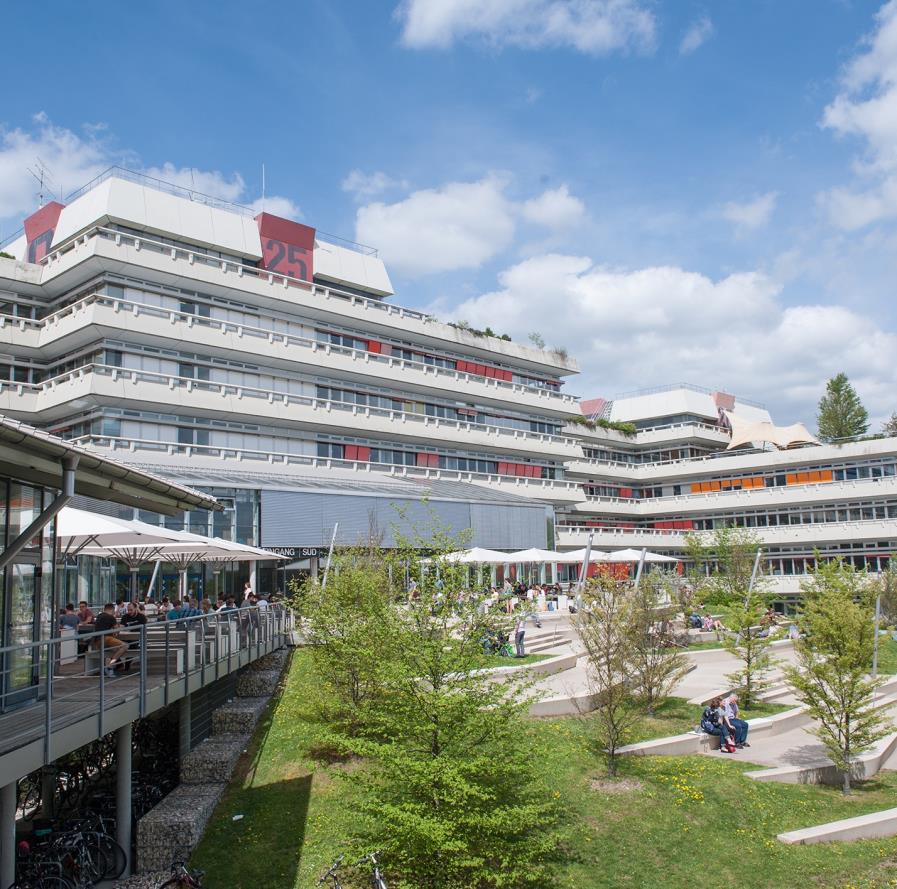
\includegraphics[width=0.455\paperwidth]{campus.png}};
  % institute label above photo
  \node[anchor=south west,font=\bfseries\small,text=uulmtitle]
    at ([xshift=0.55cm,yshift=-1.75cm]current page.north west)
    {Institut f\"ur Datenbanken und Informationssysteme};
  % right: red panel
  \fill[uulmred] ([xshift=0cm,yshift=-1.85cm]current page.north)
    rectangle ([xshift=-0.5cm,yshift=0.95cm]current page.south east);
  % title text
  \node[anchor=north west,text=white,align=left,text width=0.45\paperwidth,
        font=\bfseries]
    at ([xshift=0.35cm,yshift=-2.4cm]current page.north)
    {{\fontsize{16}{20}\selectfont Assessing the Effectiveness of Large Language Model Support for Generating GDPR ROPA Documentation}\\[1.0cm]
     {\fontsize{12}{15}\selectfont Master Thesis Presentation}\\[0.35cm]
     {\fontsize{12}{15}\selectfont Emilija Kastratovi\'c}};
\end{tikzpicture}
\end{frame}
}

% ============================================================
% 2 -- GDPR and ROPA  (+ 3 bullets)
% ============================================================
\begin{frame}{GDPR and ROPA}
\begin{columns}[T]
\begin{column}{0.64\textwidth}
\vspace{0.4cm}
\small
\begin{itemize}
  \setlength{\itemsep}{0.5cm}
  \item A \textbf{Record of Processing Activities (ROPA)} is the Article~30 GDPR
        record every organization must keep~\cite{gdpr-info-art30}: what personal data
        it processes, for which purposes, and on what legal basis.
  \item Maintaining it is \textbf{tedious and expertise-heavy}, a real burden for
        small companies that have no dedicated \textbf{Data Protection Officer (DPO)}.
  \item \textbf{LLM support} is a promising solution: it lowers the legal-knowledge
        barrier and drafts the document for non-experts.
\end{itemize}
\end{column}
\begin{column}{0.32\textwidth}
\centering

\includegraphics[height=2.5cm]{icon_gdpr.png}\\[0.6cm]

\includegraphics[height=2.5cm]{icon_ai.png}
\end{column}
\end{columns}
\srcline{GDPR~\cite{gdpr-eu-overview}; Article~30 / ROPA~\cite{gdpr-info-art30}}
\end{frame}

% ============================================================
% 3 -- Document Info and Generation
% ============================================================
\begin{frame}{Document Info and Generation}
\begin{columns}[T]
\begin{column}{0.5\textwidth}
\centering
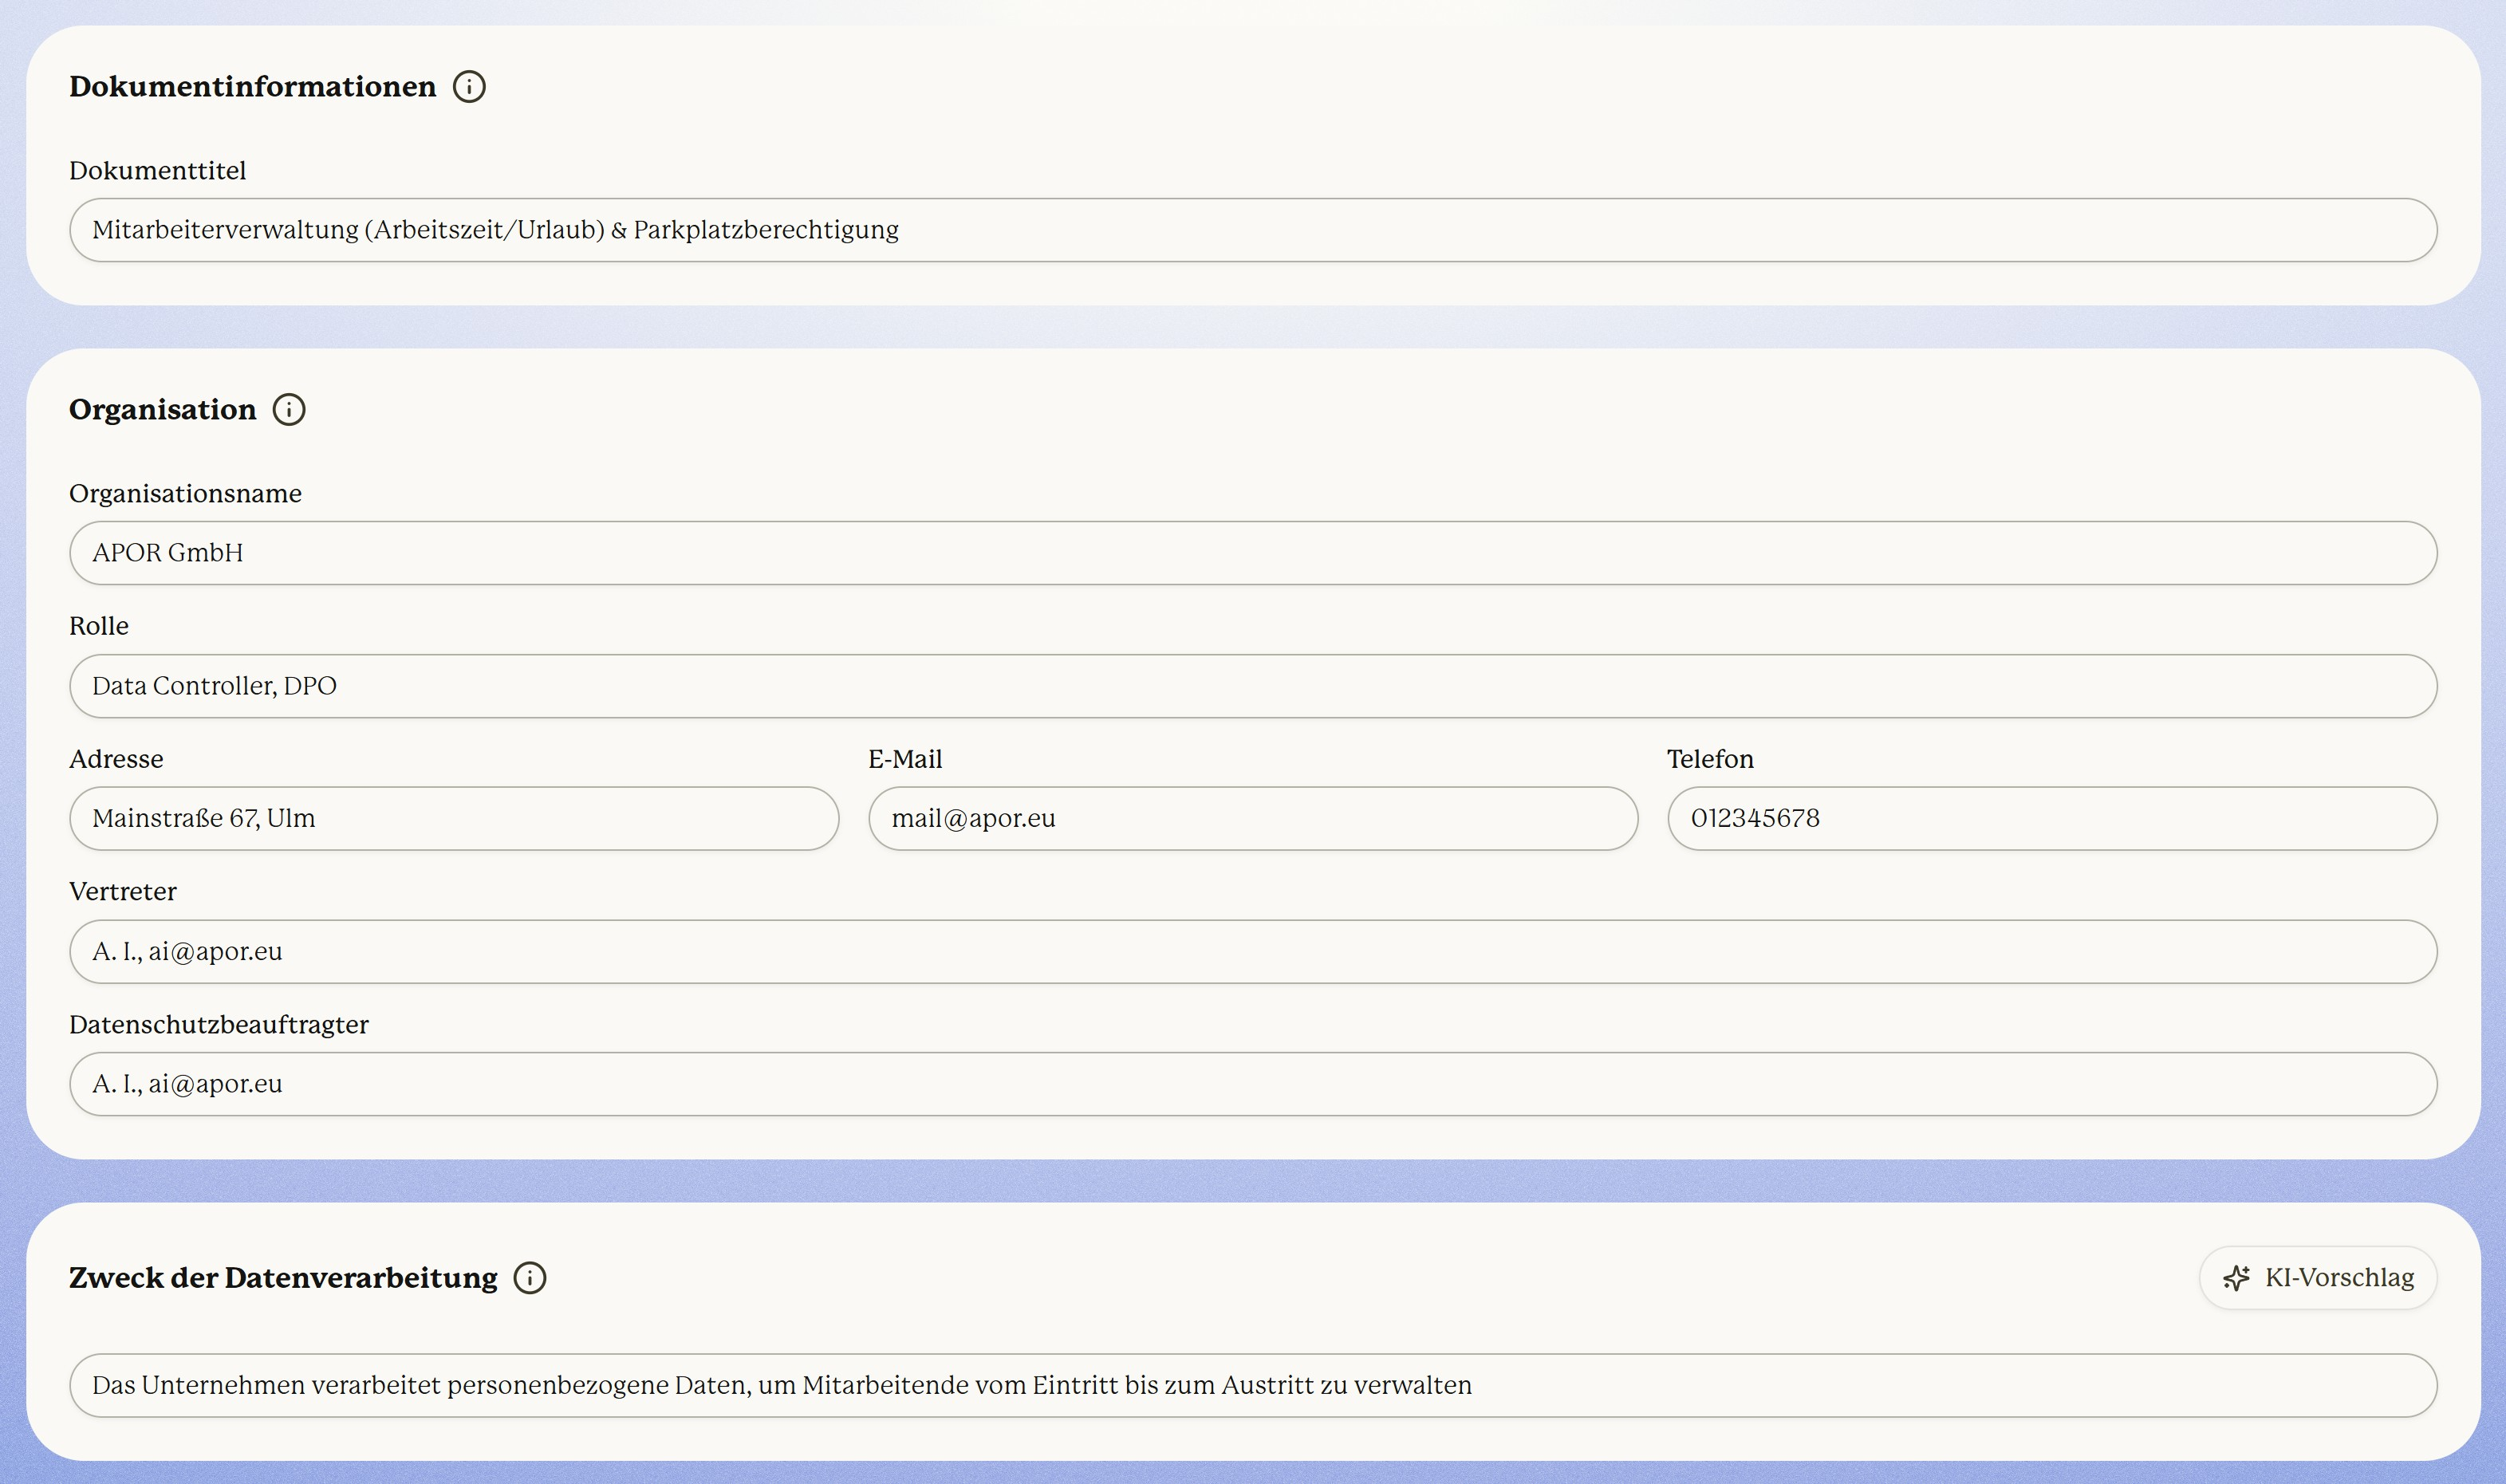
\includegraphics[width=\linewidth,height=0.68\textheight,keepaspectratio]{ropagen-intro.jpg}\\[0.15cm]
{\scriptsize Structured document and organization information}
\end{column}
\begin{column}{0.5\textwidth}
\centering
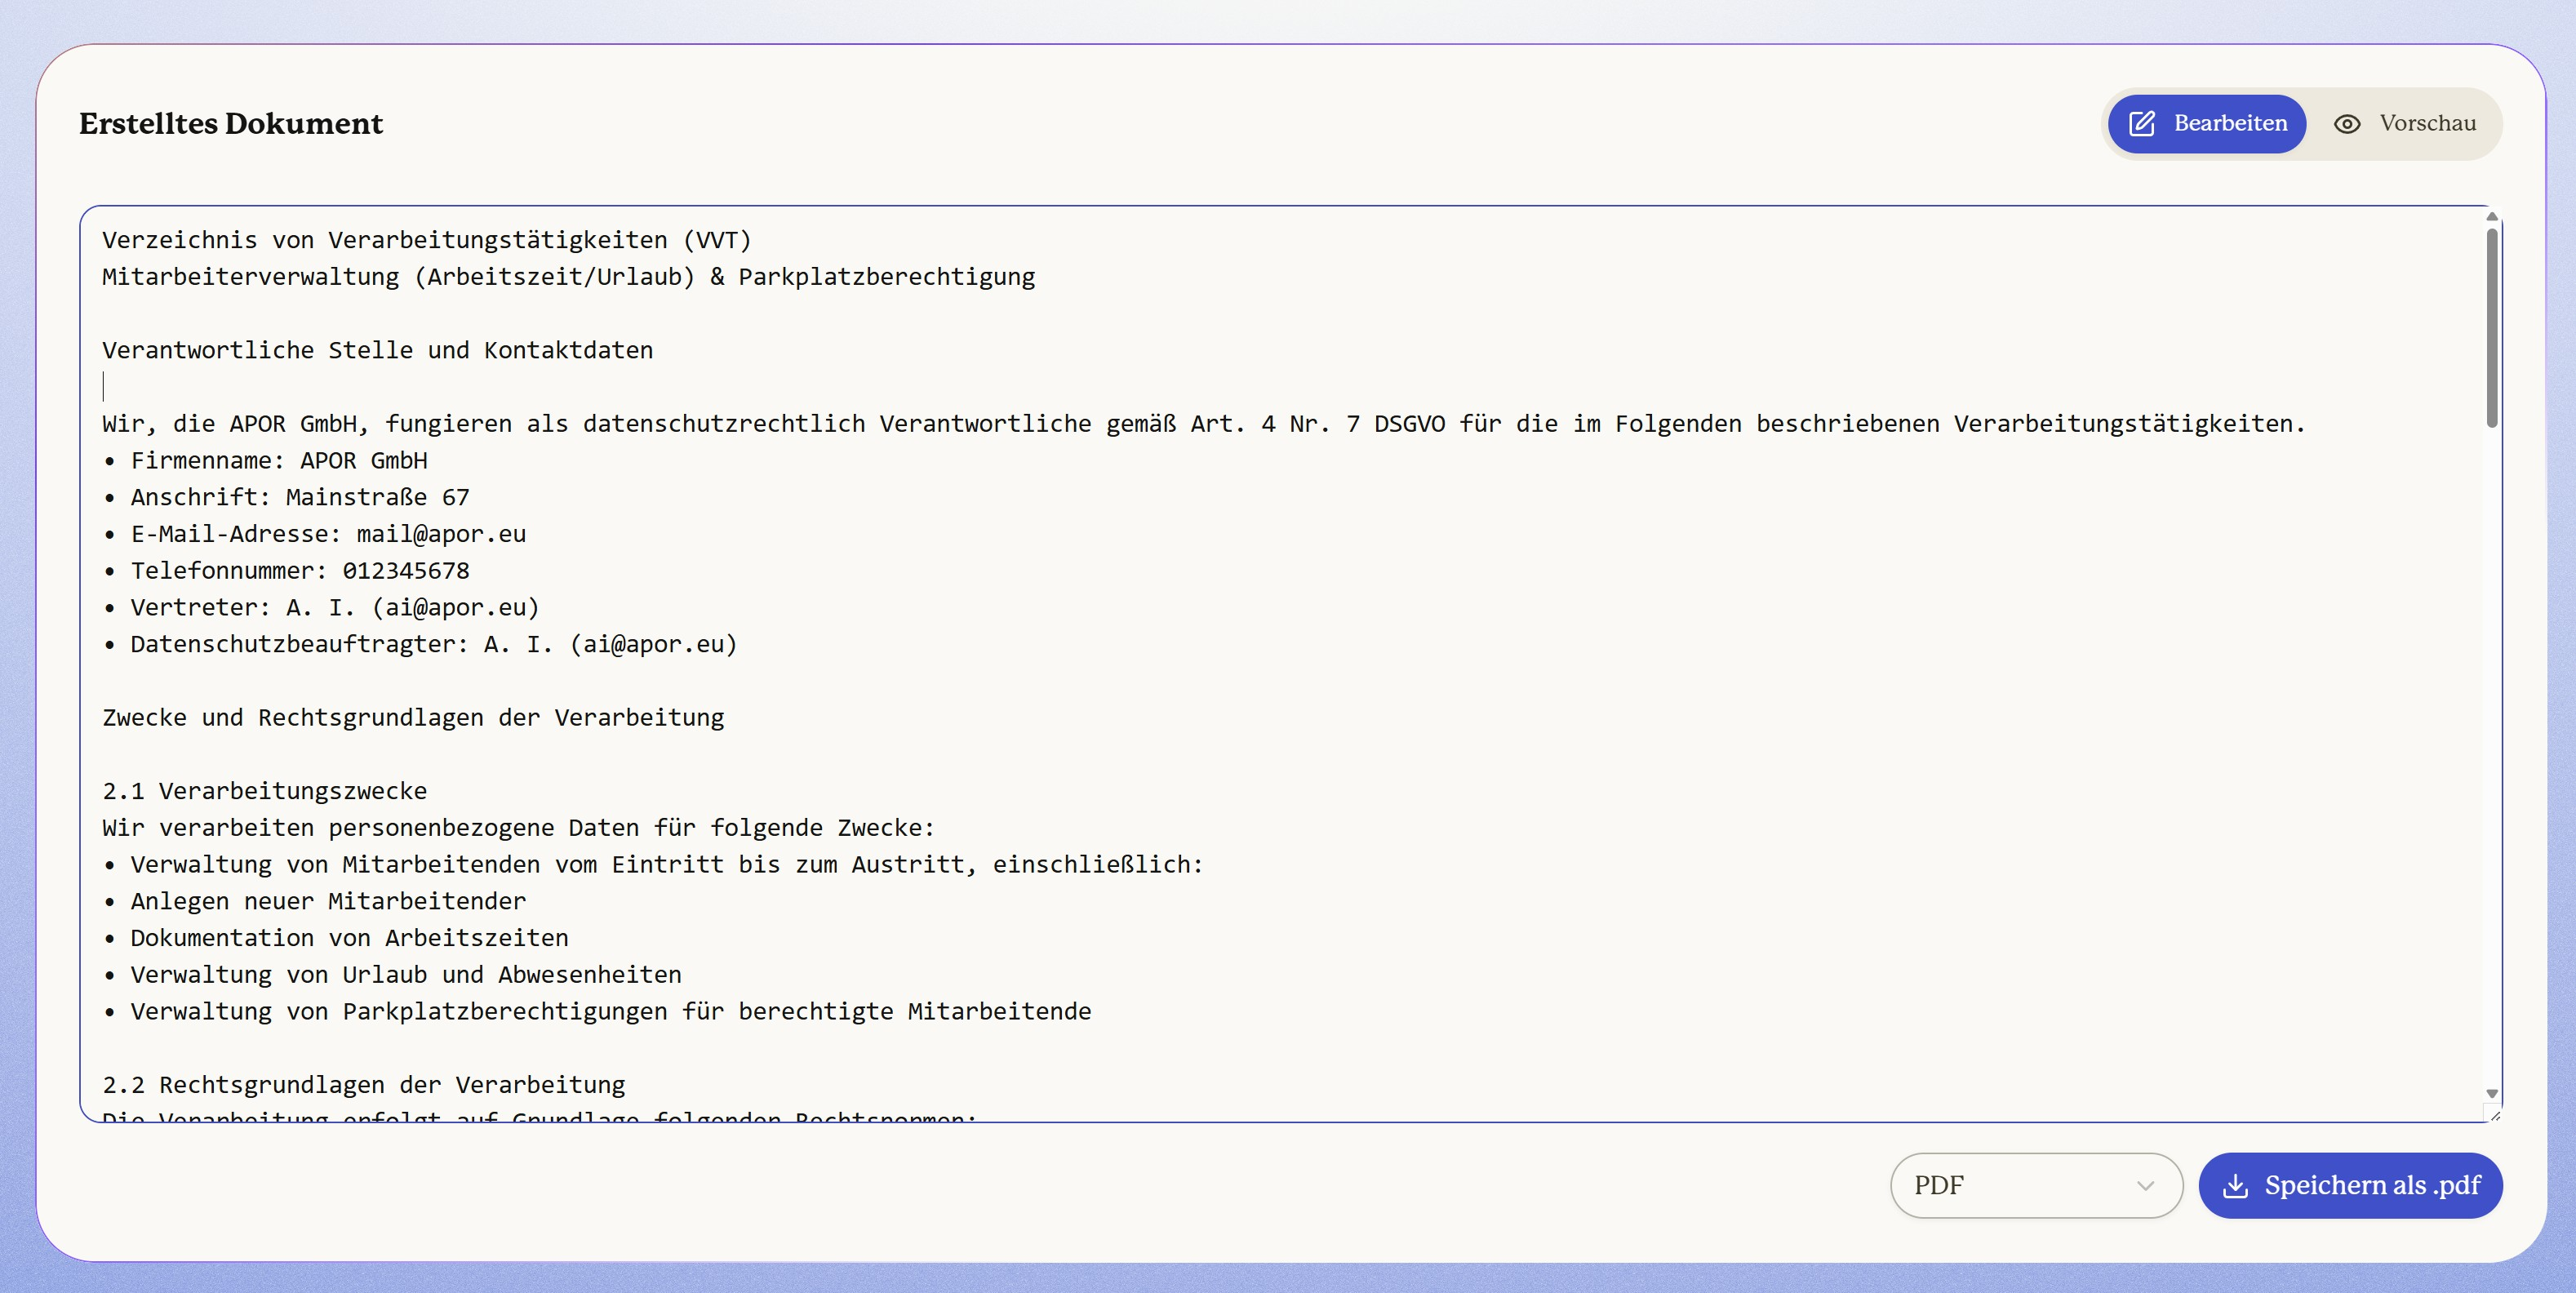
\includegraphics[width=\linewidth,height=0.68\textheight,keepaspectratio]{ropagen-generated.jpg}\\[0.15cm]
{\scriptsize The generated ROPA document}
\scriptsize
\begin{itemize}\setlength{\itemsep}{0.35cm}
    \item \textbf{Mistral} as the LLM backbone (interchangeable)
\end{itemize}
\end{column}
\end{columns}
\end{frame}

% ============================================================
% 4 -- Form Mode (+ takeaways)
% ============================================================
\begin{frame}{Form Mode -- Checkboxes}
\begin{columns}[T]
\begin{column}{0.66\textwidth}
\centering
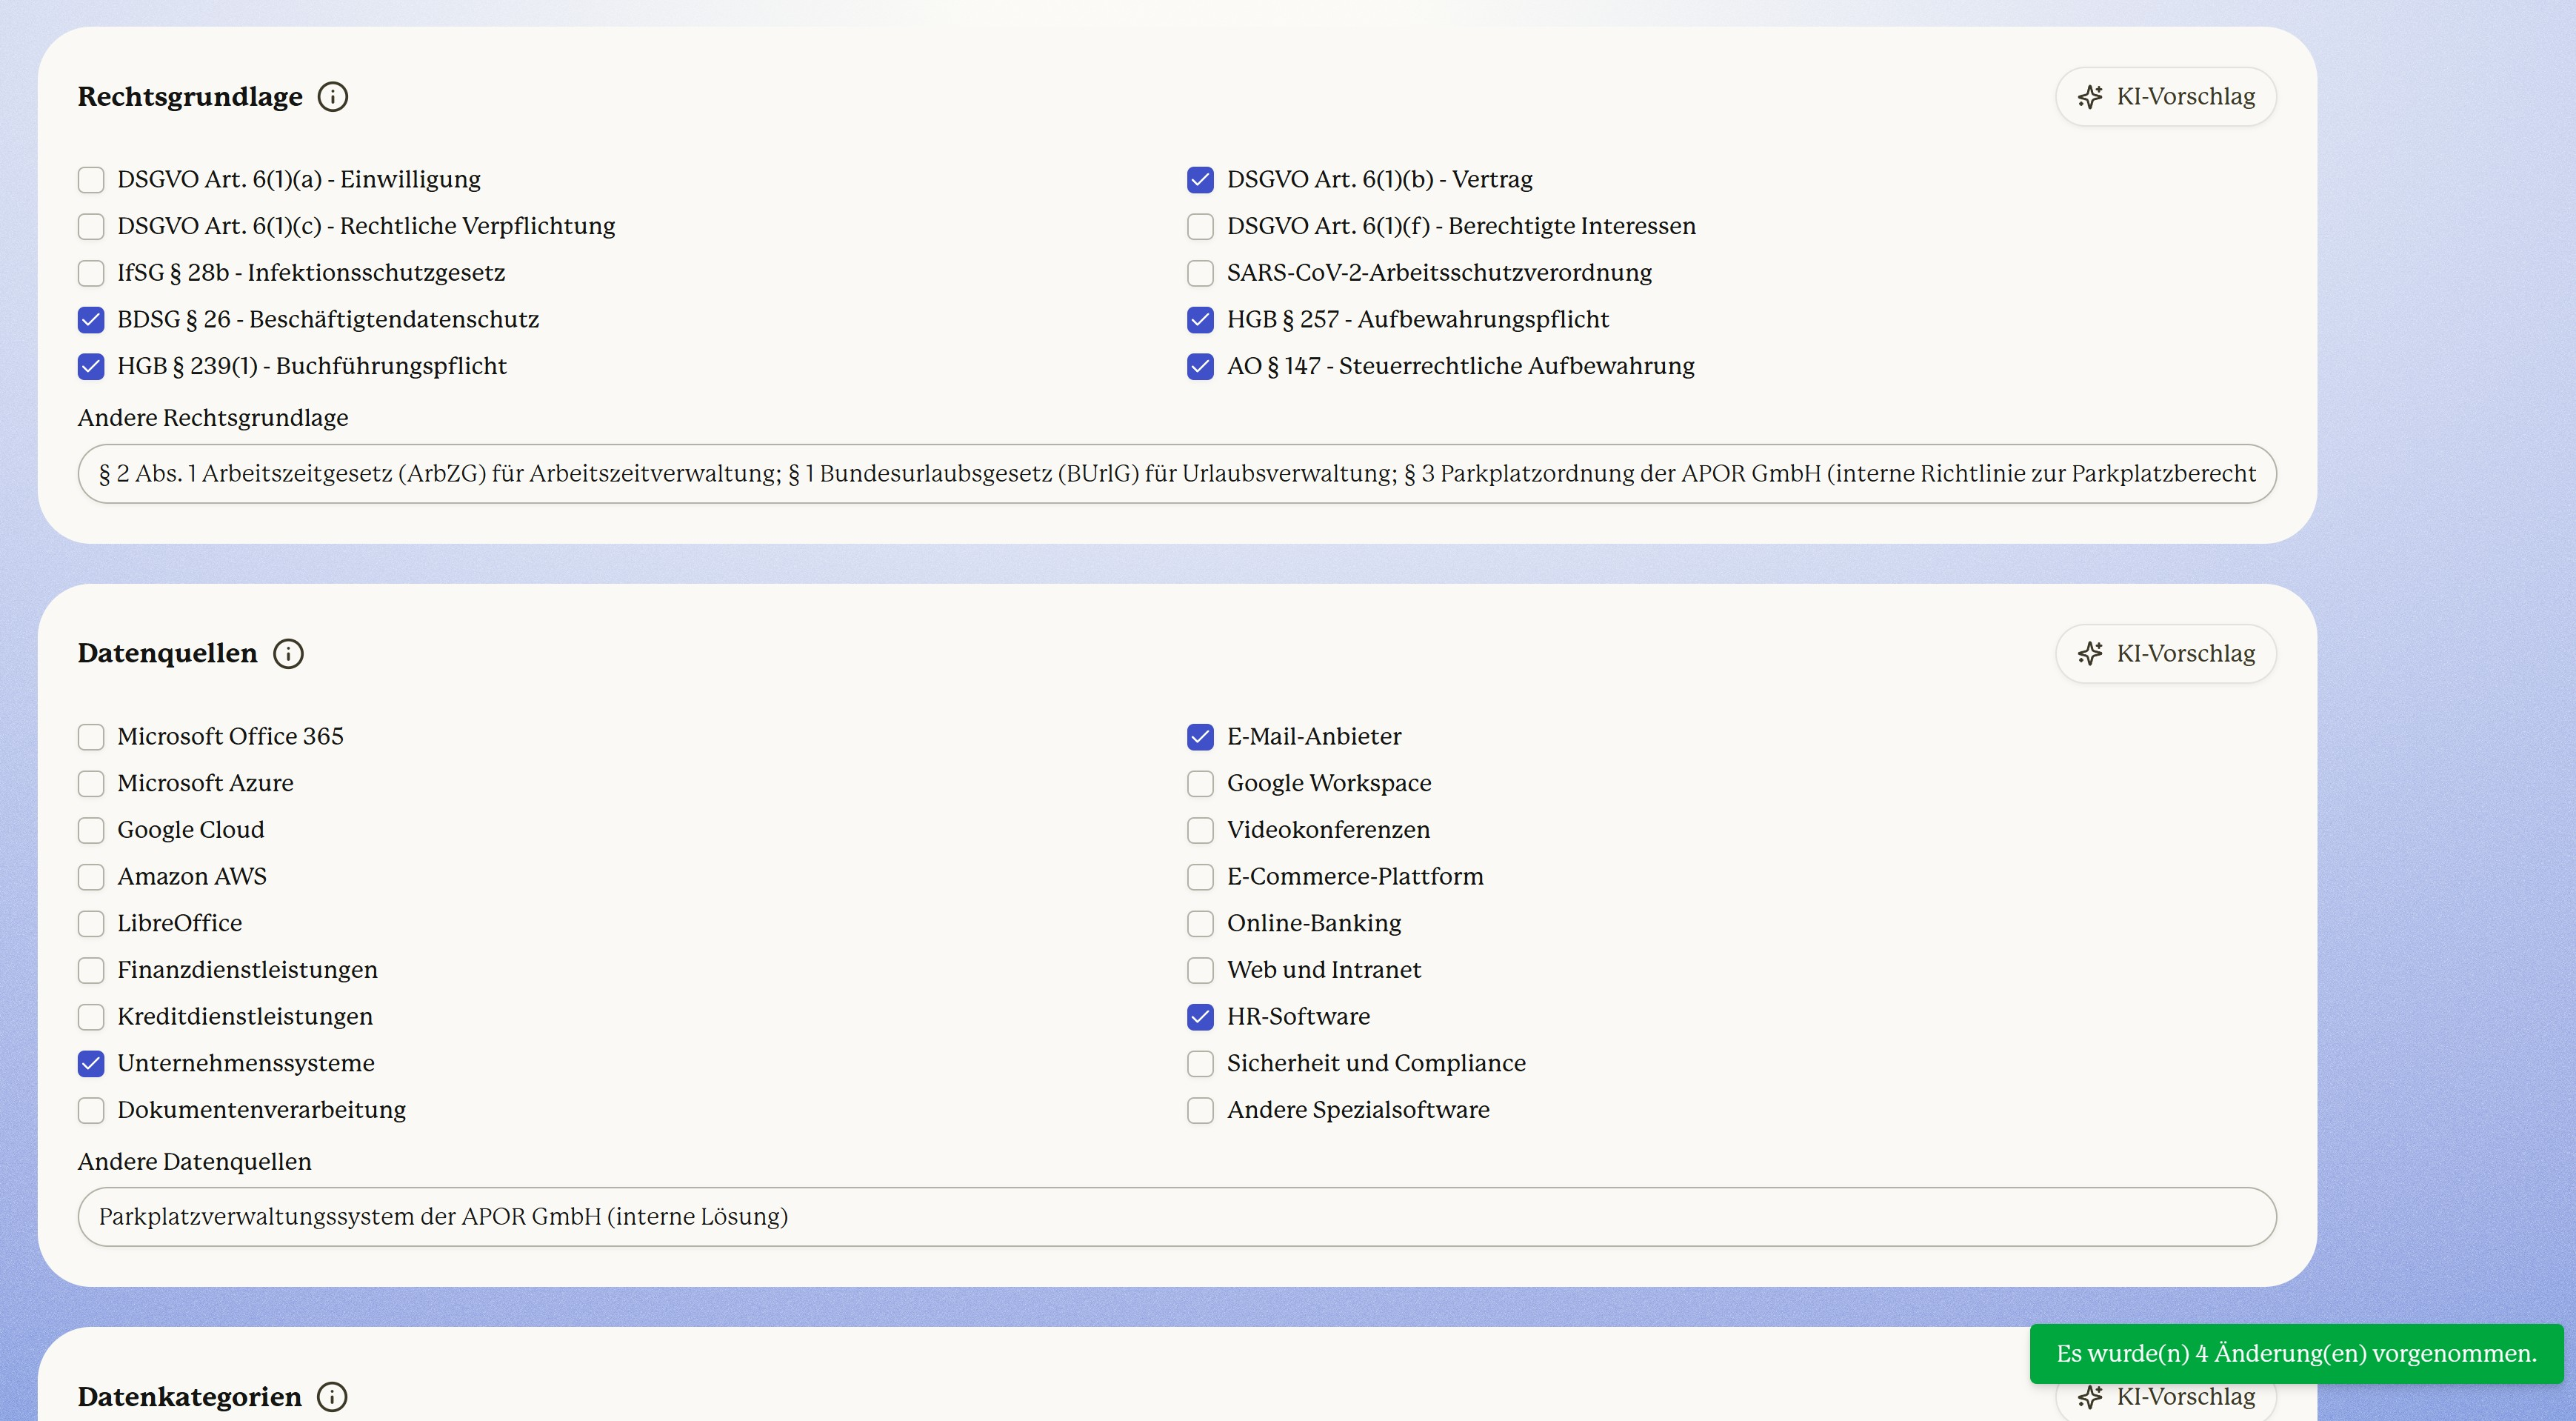
\includegraphics[width=\linewidth,height=0.74\textheight,keepaspectratio]{ropagen-form.jpg}
\end{column}
\begin{column}{0.32\textwidth}
\vspace{0.3cm}
\scriptsize
\begin{itemize}\setlength{\itemsep}{0.35cm}
  \item \textbf{Standardized fields $\rightarrow$ Form}: checkboxes fit well-defined inputs.
  \item Laid out and \textbf{dictates what to do} $\rightarrow$ clarity and control.
\end{itemize}
\end{column}
\end{columns}
\end{frame}

% ============================================================
% 5 -- Ask Mode (+ takeaways)
% ============================================================
\begin{frame}{Ask Mode -- Hybrid}
\begin{columns}[T]
\begin{column}{0.66\textwidth}
\centering
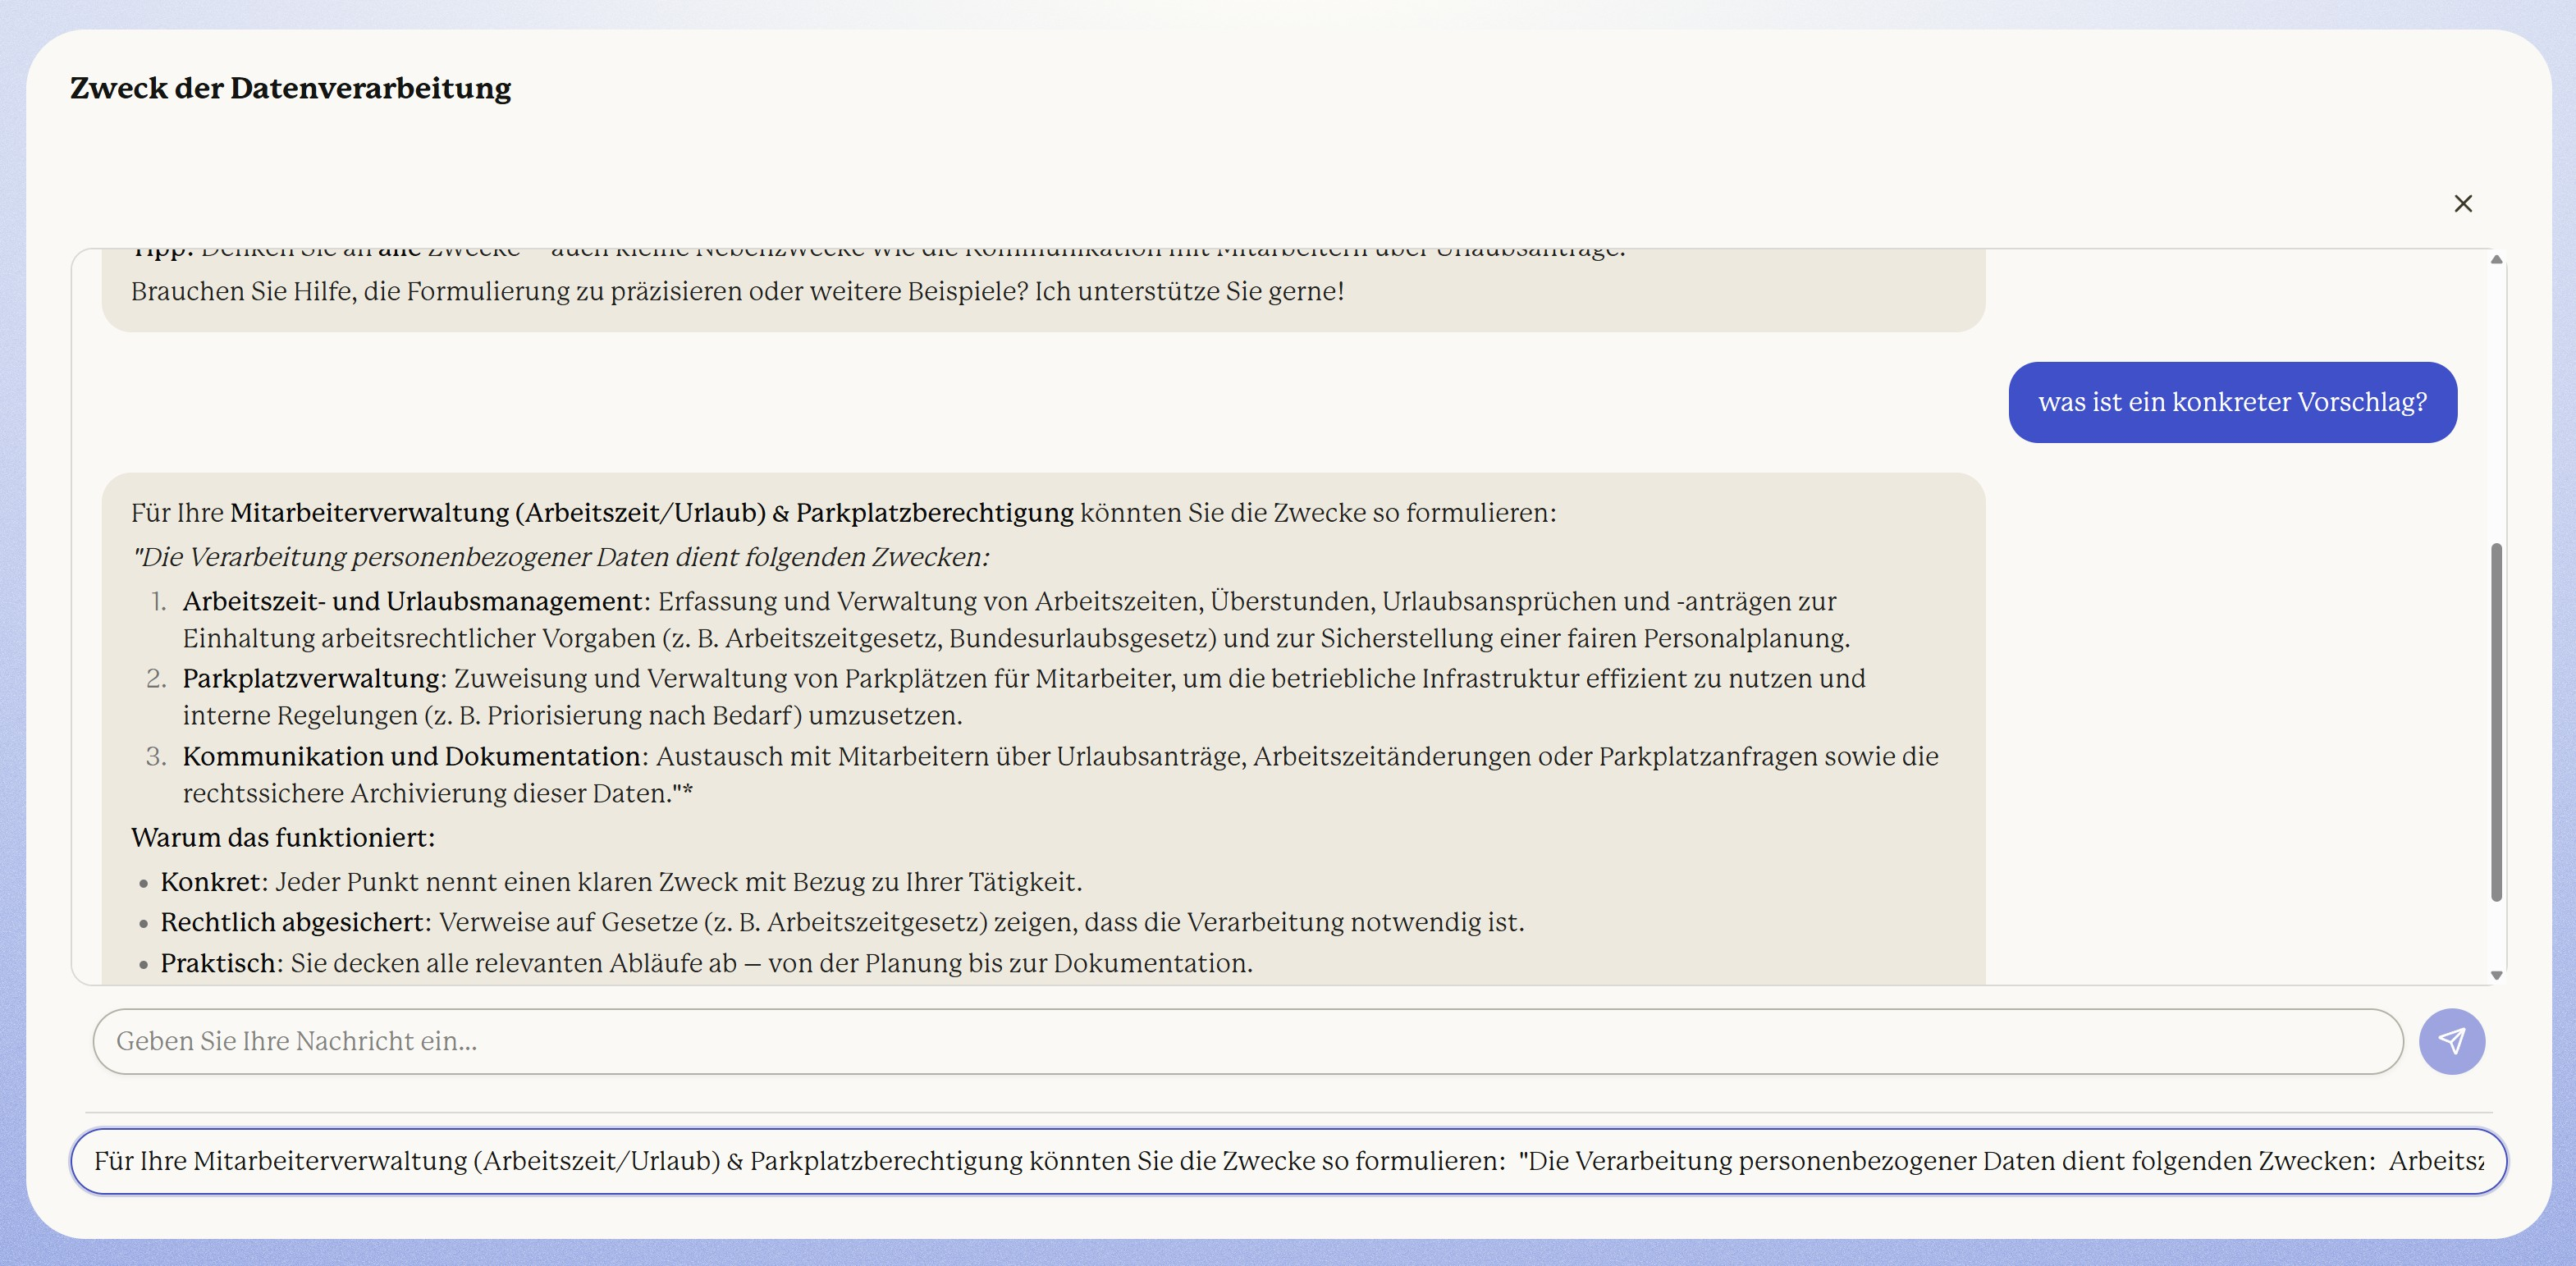
\includegraphics[width=\linewidth,height=0.74\textheight,keepaspectratio]{ropagen-ask.jpg}
\end{column}
\begin{column}{0.32\textwidth}
\vspace{0.3cm}
\scriptsize
\begin{itemize}\setlength{\itemsep}{0.4cm}
  \item \textbf{Most transparent} mode: the user sees every step.
  \item But the user must \textbf{look out for everything}.
\end{itemize}
\end{column}
\end{columns}
\end{frame}

% ============================================================
% 6 -- Chat Mode (+ takeaways)
% ============================================================
\begin{frame}{Chat Mode -- Autonomous LLM}
\begin{columns}[T]
\begin{column}{0.66\textwidth}
\centering
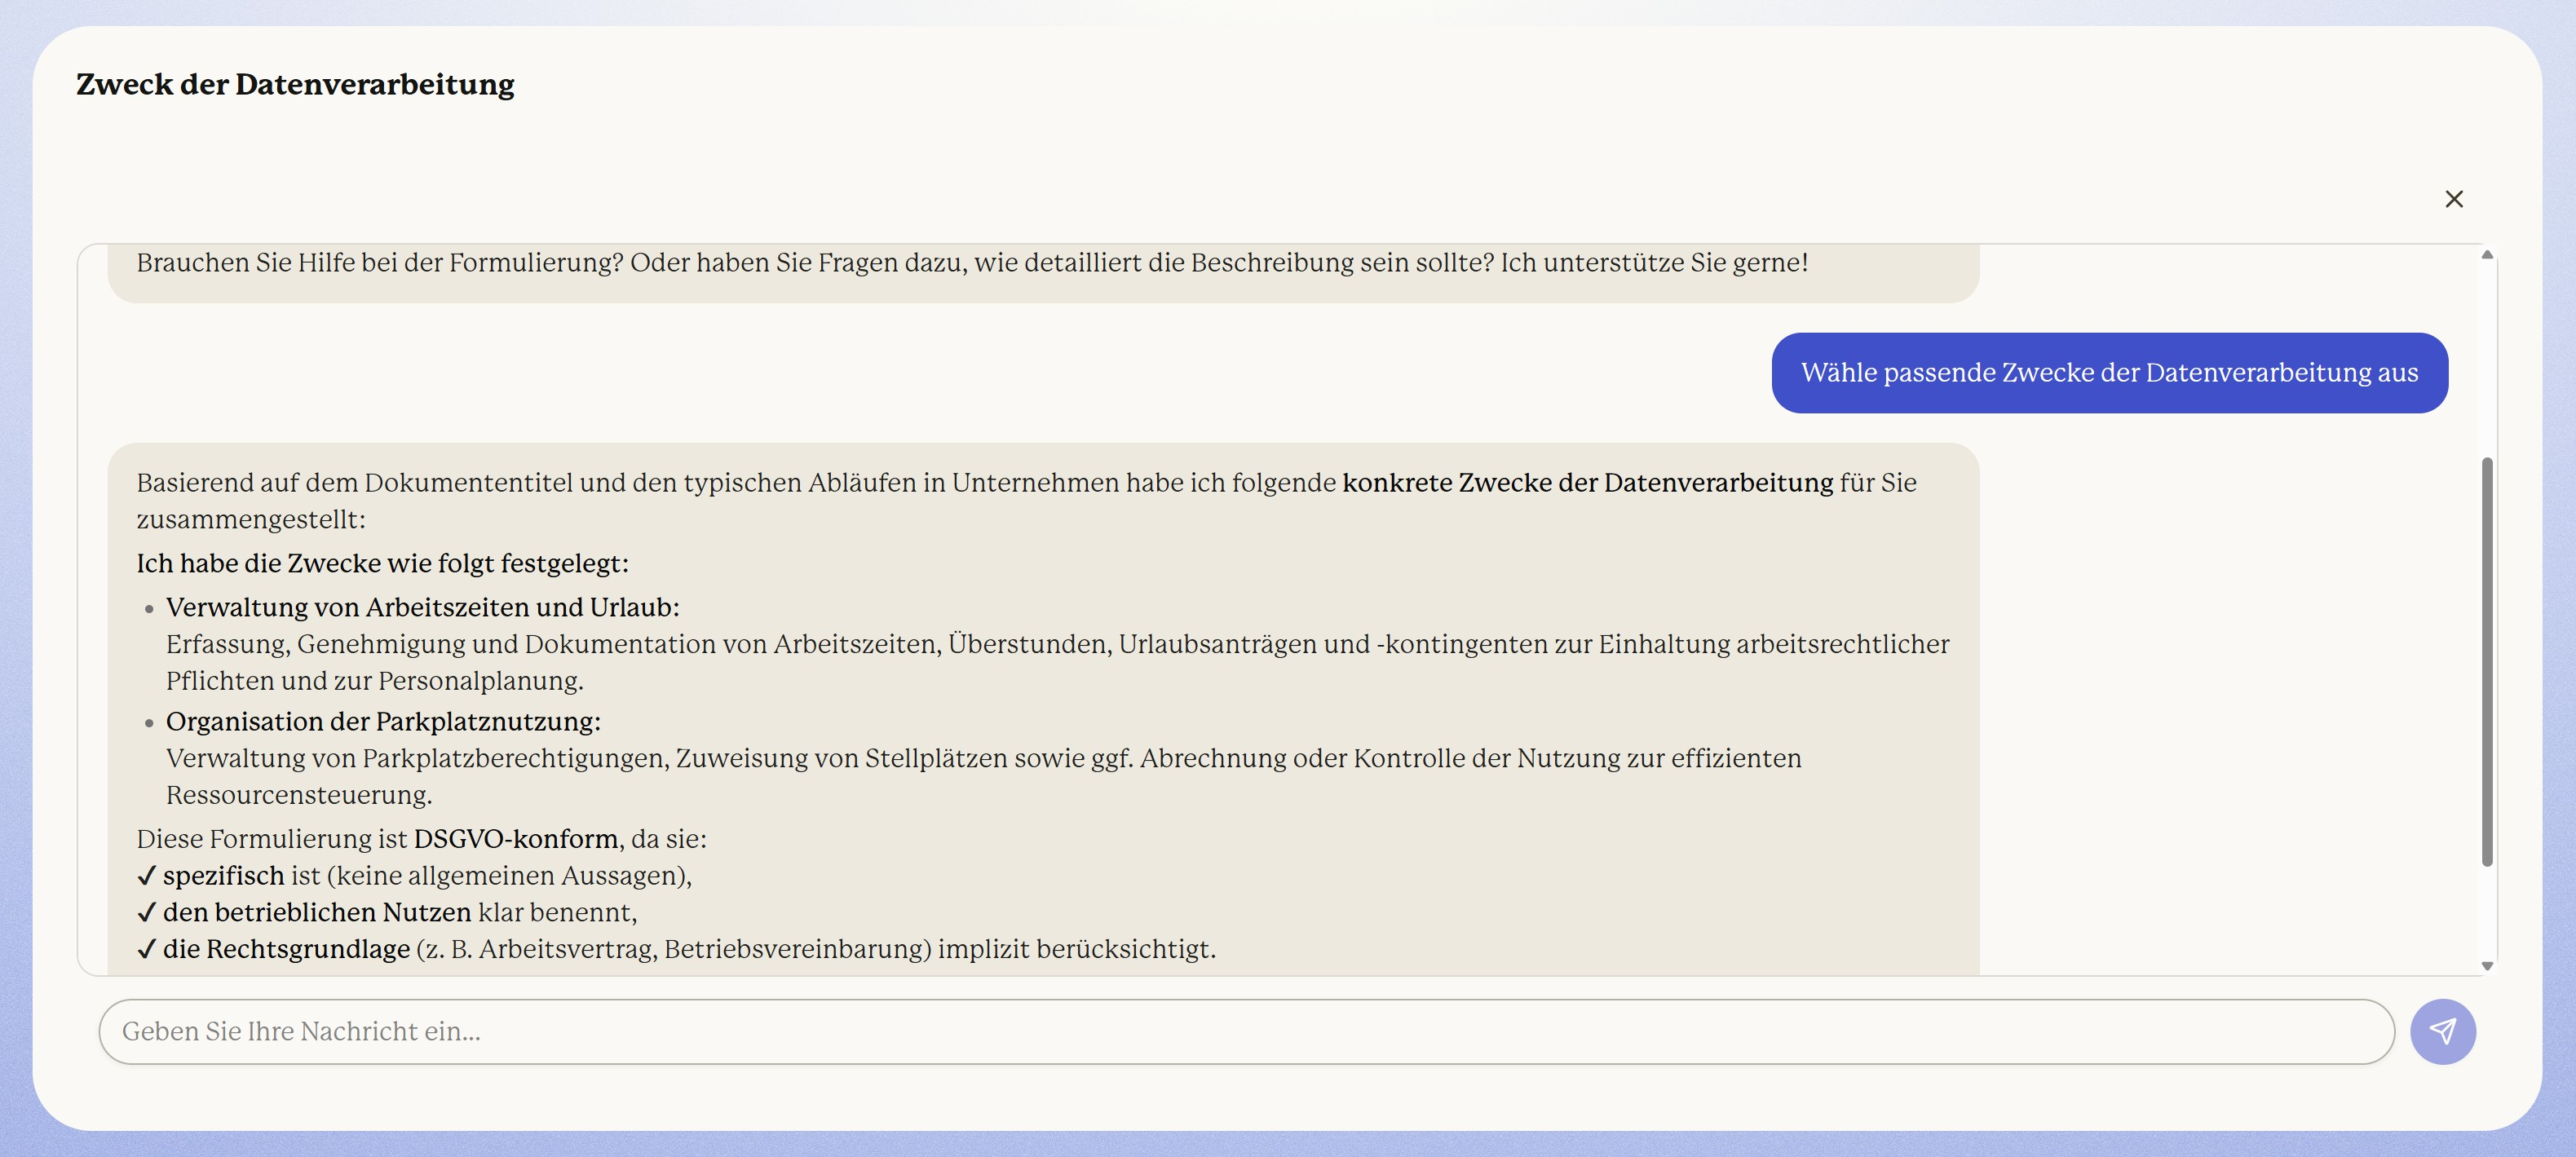
\includegraphics[width=\linewidth,height=0.74\textheight,keepaspectratio]{ropagen-chat.jpg}
\end{column}
\begin{column}{0.32\textwidth}
\vspace{0.3cm}
\scriptsize
\begin{itemize}\setlength{\itemsep}{0.4cm}
  \item \textbf{Specific, free-form input $\rightarrow$ Chat}: open conversation fits unstructured descriptions.
  \item The LLM \textbf{takes over authorship} (autonomous).
  \item Least overhead, least direct control.
\end{itemize}
\end{column}
\end{columns}
\end{frame}

% ============================================================
% 7 -- RQ1 divider
% ============================================================
\begin{frame}
\rqband{\rqbody{white}{rqfade}{rqfade}}
\end{frame}

% ============================================================
% 8 -- Study Scenario
% ============================================================
\begin{frame}{Study Scenario}
\centering
\vspace{0.15cm}
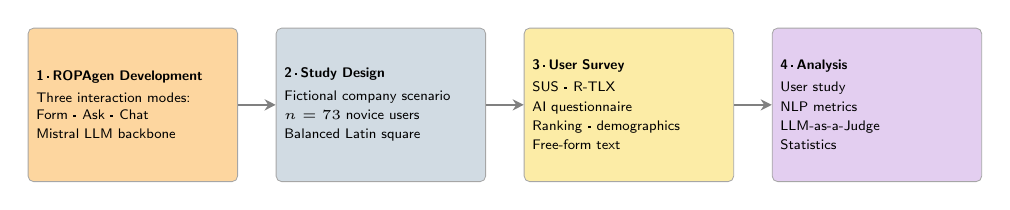
\begin{tikzpicture}[font=\tiny,
  tlbox/.style={rectangle, rounded corners=2pt, draw=black!35, line width=0.3pt,
    text width=2.45cm, inner sep=3pt, align=left, anchor=north west, minimum height=1.95cm},
  tlarr/.style={-{Stealth[length=4pt,width=4pt]}, line width=0.9pt, color=black!50}]
  \node[tlbox, fill=uulmgold!50] (b1) at (0,0)
    {\textbf{1\,\textperiodcentered\,ROPAgen Development}\\[2pt]
     Three interaction modes:\\ Form \textperiodcentered\ Ask \textperiodcentered\ Chat\\[1pt] Mistral LLM backbone};
  \node[tlbox, fill=uulmblue!35] (b2) at (3.15,0)
    {\textbf{2\,\textperiodcentered\,Study Design}\\[2pt]
     Fictional company scenario\\[1pt] $n=73$ novice users\\[1pt] Balanced Latin square};
  \node[tlbox, fill=tlYellow] (b3) at (6.30,0)
    {\textbf{3\,\textperiodcentered\,User Survey}\\[2pt]
     SUS \textperiodcentered\ R-TLX\\[1pt] AI questionnaire\\[1pt] Ranking \textperiodcentered\ demographics\\[1pt] Free-form text};
  \node[tlbox, fill=tlPurple] (b4) at (9.45,0)
    {\textbf{4\,\textperiodcentered\,Analysis}\\[2pt]
     User study\\[1pt] NLP metrics\\[1pt] LLM-as-a-Judge\\[1pt] Statistics};
  \draw[tlarr] (b1.east) -- (b2.west);
  \draw[tlarr] (b2.east) -- (b3.west);
  \draw[tlarr] (b3.east) -- (b4.west);
\end{tikzpicture}\\[0.4cm]
\begin{columns}[T]
\begin{column}{0.5\textwidth}\centering
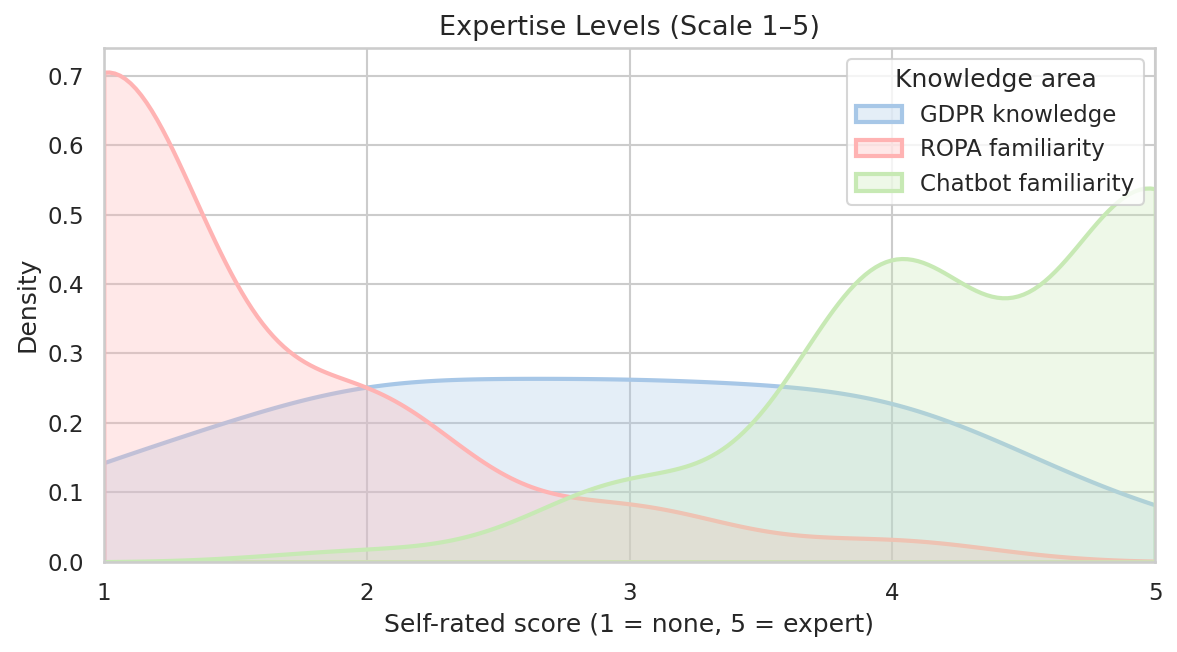
\includegraphics[width=\linewidth,height=0.46\textheight,keepaspectratio]{demographics_expertise.png}
\end{column}
\begin{column}{0.5\textwidth}\centering
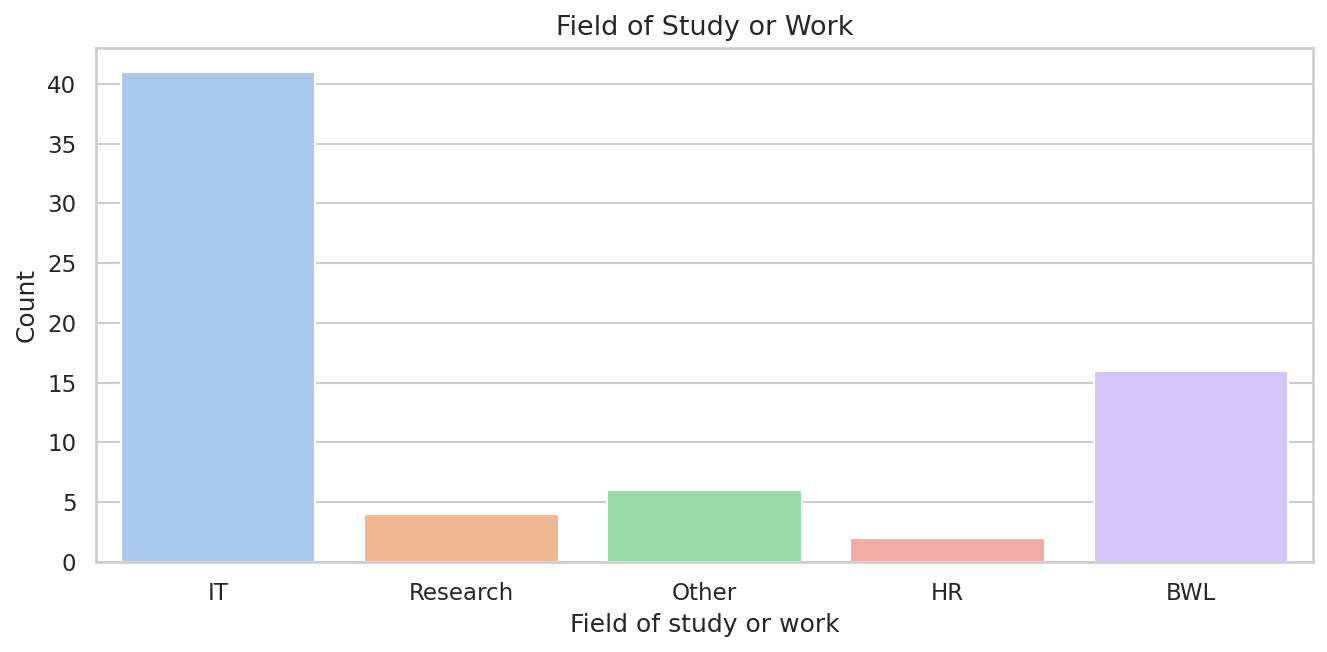
\includegraphics[width=\linewidth,height=0.46\textheight,keepaspectratio]{demographics_field.png}
\end{column}
\end{columns}
\srcline{Study design \& non-parametric analysis~\cite{SauroLewis2016}}
\end{frame}

% ============================================================
% 9 -- SUS Results (bar chart + item table)
% ============================================================
\begin{frame}{System Usability Score Results}
\begin{columns}[c]
\begin{column}{0.44\textwidth}\centering
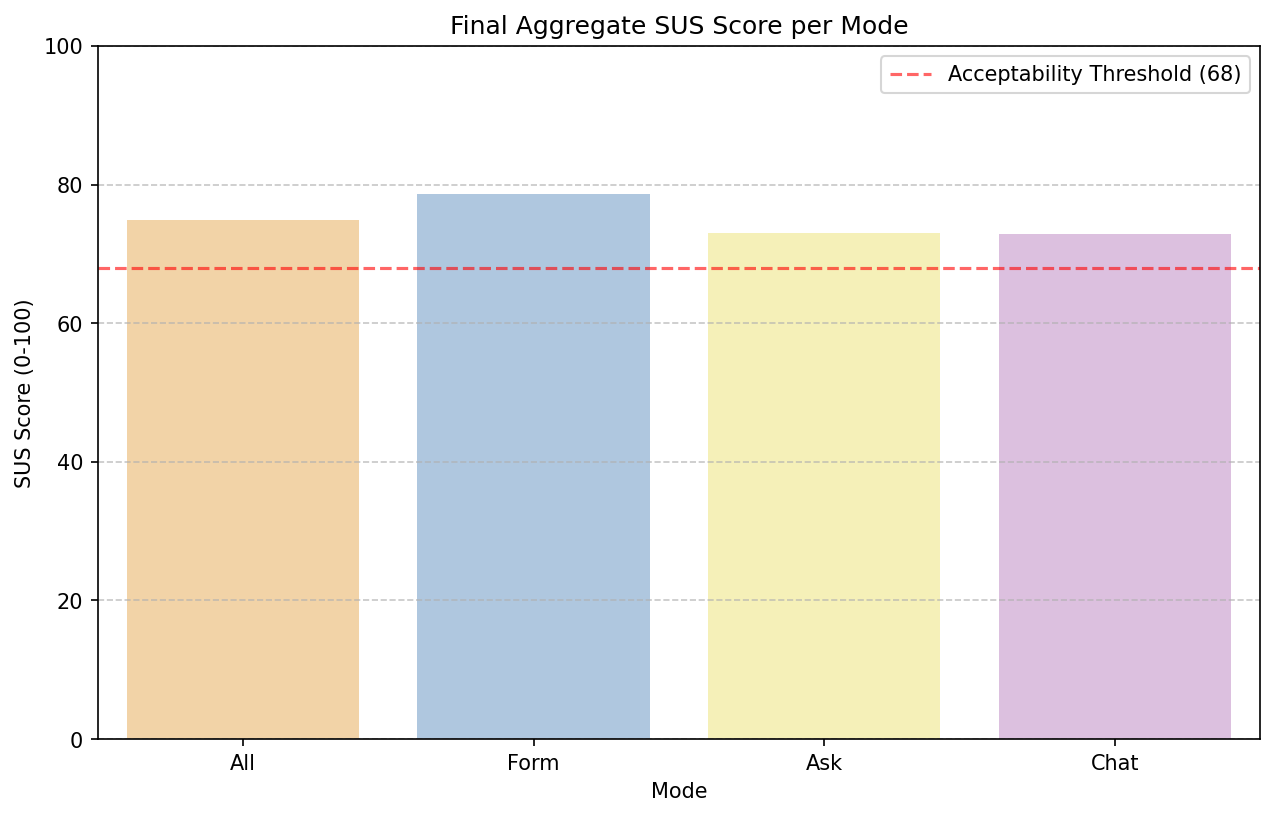
\includegraphics[width=\linewidth,height=0.72\textheight,keepaspectratio]{sus_aggregate_barplot.png}
\end{column}
\begin{column}{0.56\textwidth}
\centering
\setlength{\tabcolsep}{6pt}\renewcommand{\arraystretch}{1.05}
\scriptsize
\begin{tabular}{@{}c p{4.4cm} ccc@{}}
\toprule
\# & Item & Form & Ask & Chat\\
\midrule
1 & I think that I would like to use this system frequently. & \textbf{3.52} & 3.22 & 3.22\\
2 & I found the system unnecessarily complex. & \textbf{1.64} & 2.25 & 2.12\\
3 & I thought the system was easy to use. & \textbf{4.38} & 4.01 & 3.99\\
4 & I think I would need the support of a technical person to use this system. & 1.52 & \textbf{1.49} & 1.55\\
5 & I found the various functions in this system were well integrated. & \textbf{4.00} & 3.67 & 3.64\\
6 & I thought there was too much inconsistency in this system. & 2.16 & 2.04 & \textbf{2.01}\\
7 & I would imagine that most people would learn to use this system very quickly. & \textbf{4.30} & 4.00 & 4.03\\
8 & I found the system very cumbersome to use. & \textbf{1.65} & 2.16 & 2.29\\
9 & I felt very confident using the system. & 3.83 & 3.84 & \textbf{3.90}\\
10 & I needed to learn a lot of things before I could get going. & \textbf{1.61} & 1.61 & 1.62\\
\bottomrule
\end{tabular}
\end{column}
\end{columns}
\srcline{System Usability Scale (SUS)~\cite{Brooke1996}}
\end{frame}

% ============================================================
% 10 -- NASA R-TLX + completion time
% ============================================================
\begin{frame}{NASA R-TLX and Per-Mode Completion Time}
\begin{columns}[T]
\begin{column}{0.56\textwidth}
\centering
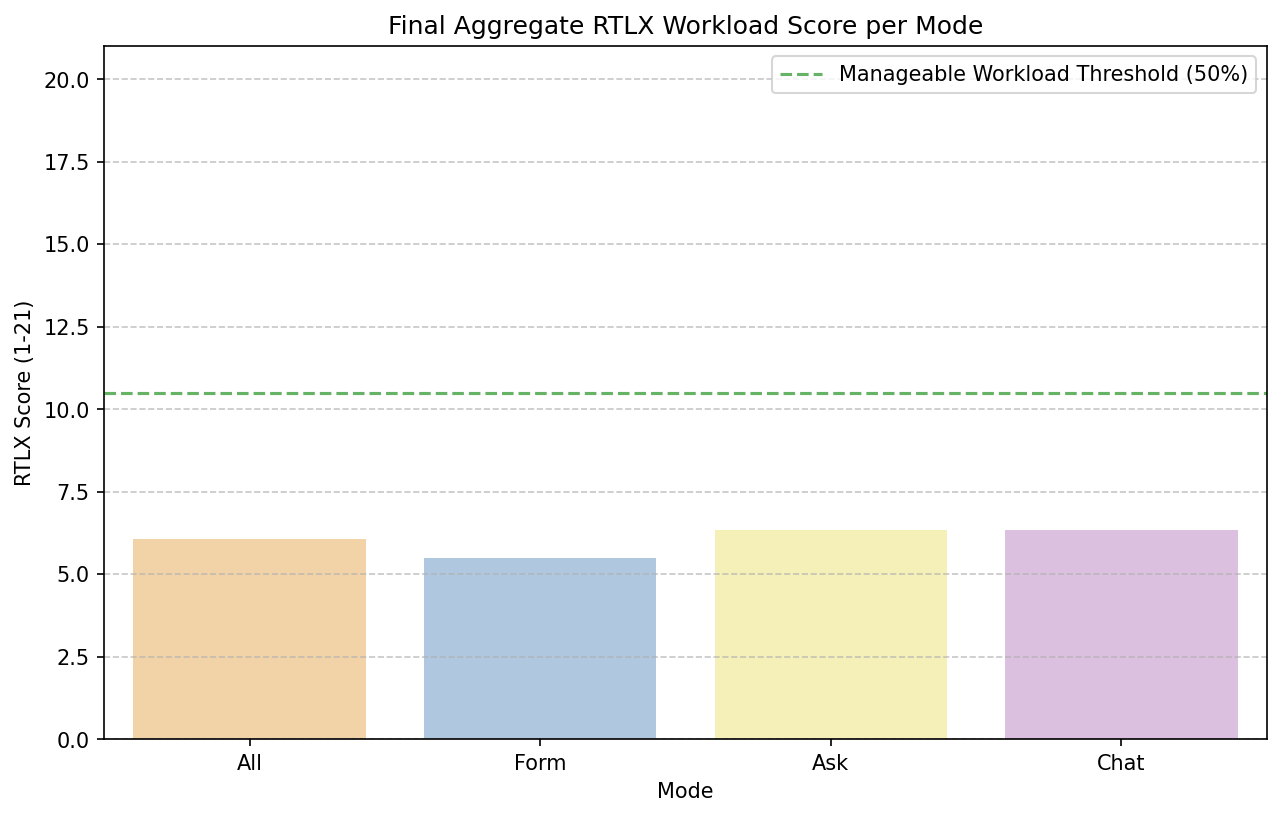
\includegraphics[width=0.82\linewidth,height=0.40\textheight,keepaspectratio]{rtlx_aggregate_barplot.png}\\[0.2cm]
\setlength{\tabcolsep}{6pt}\renewcommand{\arraystretch}{1.1}
\scriptsize
\begin{tabular}{@{}l ccc@{}}
\toprule
Subscale & Form & Ask & Chat\\
\midrule
Mental Demand    & \textbf{5.77} & 6.80 & 6.36\\
Physical Demand  & \textbf{2.77} & 3.54 & 3.26\\
Temporal Demand  & \textbf{4.16} & 4.97 & 5.54\\
Effort           & \textbf{5.68} & 6.39 & 6.32\\
Frustration      & \textbf{5.88} & 7.58 & 7.13\\
Performance (pos.) & 8.71 & \textbf{8.68} & 9.39\\
\bottomrule
\end{tabular}
\end{column}
\begin{column}{0.44\textwidth}
\centering
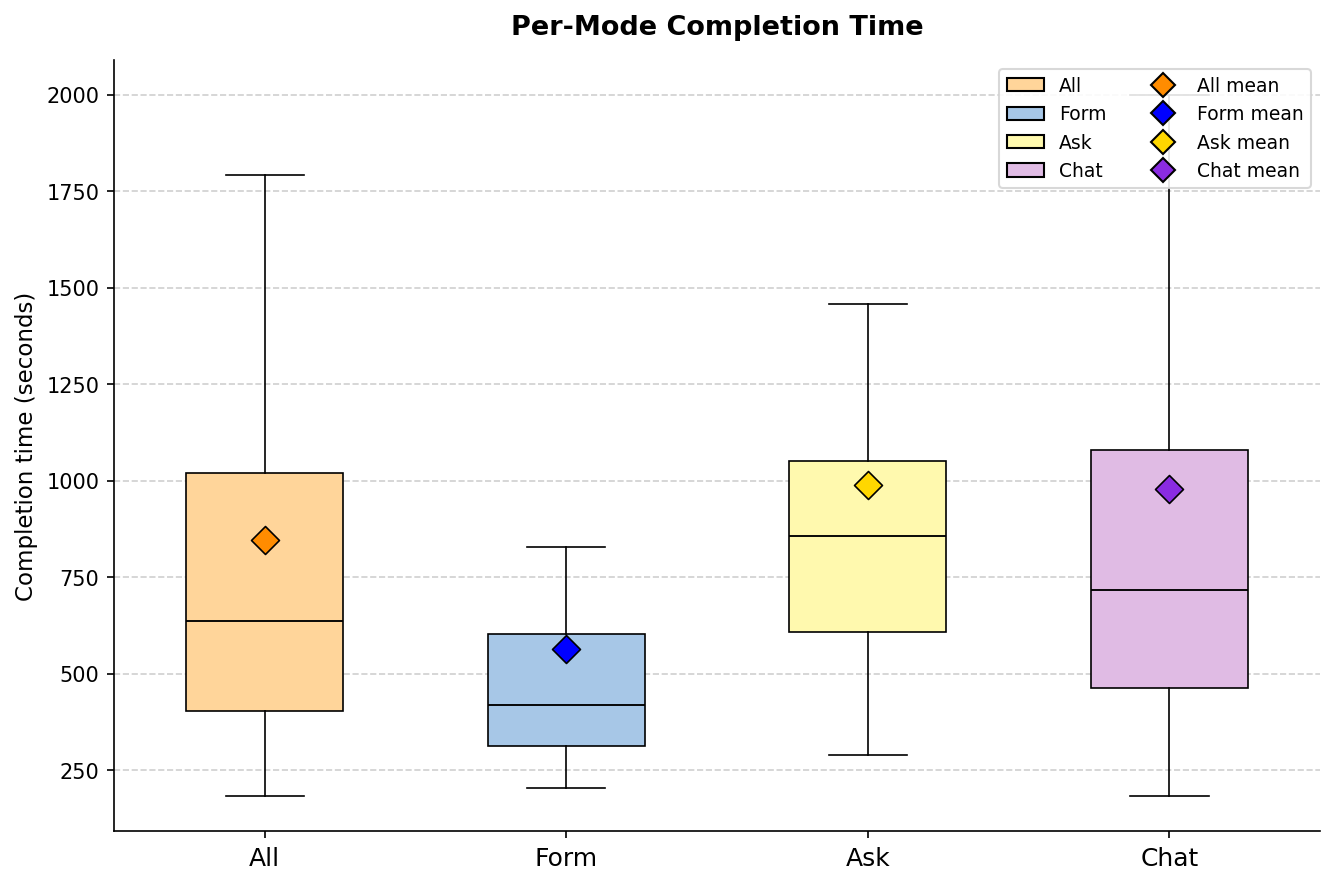
\includegraphics[width=\linewidth,height=0.72\textheight,keepaspectratio]{per_mode_timing_boxplot.png}
\end{column}
\end{columns}
\srcline{NASA Raw Task Load Index (R-TLX)~\cite{Hart1988,Hart2006}}
\end{frame}

% ============================================================
% 11 -- Mode Ranking
% ============================================================
\begin{frame}{Mode Ranking}
\centering
\setlength{\tabcolsep}{14pt}\renewcommand{\arraystretch}{1.25}
\large
\begin{tabular}{@{}l c c c@{}}
\toprule
Mode & Rank-1 votes & Share & Mean rank\\
\midrule
Form & \textbf{37} & \textbf{53.6\,\%} & \textbf{1.78}\\
Chat & 20 & 29.0\,\% & 2.07\\
Ask  & 12 & 17.4\,\% & 2.14\\
\bottomrule
\end{tabular}

\vspace{0.7cm}
\normalsize
\begin{columns}[T]
\begin{column}{0.3\textwidth}
\colorbox{uulmblue!25}{\parbox[t][2.7cm][t]{\linewidth}{\centering\textbf{1.\ Form}\\[0.3cm]
\raggedright\footnotesize \plus speed\\ \plus clarity\\ \plus control\\ \minus LLM ``guesses''}}
\end{column}
\begin{column}{0.3\textwidth}
\colorbox{uulmred!18}{\parbox[t][2.7cm][t]{\linewidth}{\centering\textbf{2.\ Chat}\\[0.3cm]
\raggedright\footnotesize \plus comfort (``LLM takes care of it'')\\ \minus LLM opacity}}
\end{column}
\begin{column}{0.3\textwidth}
\colorbox{uulmgold!30}{\parbox[t][2.7cm][t]{\linewidth}{\centering\textbf{3.\ Ask}\\[0.3cm]
\raggedright\footnotesize \plus high transparency\\ \minus cumbersome workflow}}
\end{column}
\end{columns}
\end{frame}

% ============================================================
% 12 -- RQ2 divider
% ============================================================
\begin{frame}
\rqband{\rqbody{rqfade}{white}{rqfade}}
\end{frame}

% ============================================================
% 13 -- NLP metrics (Document)  (+ precision/recall note)
% ============================================================
\begin{frame}{NLP metrics (Document)}
\centering
\setlength{\tabcolsep}{12pt}\renewcommand{\arraystretch}{1.15}
\small
\begin{tabular}{@{}l ccc@{}}
\toprule
Metric & Form & Ask & Chat\\
\midrule
BLEU    & 0.129 & 0.127 & \textbf{0.143}\\
ROUGE-1 & 0.488 & 0.465 & \textbf{0.511}\\
ROUGE-2 & \textbf{0.306} & 0.257 & 0.291\\
ROUGE-L & 0.388 & 0.347 & \textbf{0.389}\\
METEOR  & \textbf{0.412} & 0.365 & 0.390\\
\midrule
BERTScore Precision & 0.889 & 0.886 & \textbf{0.895}\\
BERTScore Recall    & \textbf{0.923} & 0.908 & 0.913\\
BERTScore F1        & \textbf{0.905} & 0.897 & 0.904\\
SBERT (ModernBERT)  & 0.986 & 0.986 & \textbf{0.990}\\
\bottomrule
\end{tabular}

\vspace{0.5cm}
\begin{minipage}{0.9\linewidth}\footnotesize\raggedright
\textbf{Precision--recall trade-off:} favoring precision risks \emph{omitting} important
content; favoring recall adds \emph{overhead}. Form and Chat lead on overlap metrics, Ask
trails: reference-based NLP alone names no decisive winner.
\end{minipage}
\srcline{BLEU~\cite{Papineni2002}; ROUGE~\cite{Lin2004}; METEOR~\cite{Banerjee2005}; BERTScore~\cite{Zhang2020}; SBERT~\cite{Reimers2019}}
\end{frame}

% ============================================================
% 14 -- RQ3 divider
% ============================================================
\begin{frame}
\rqband{\rqbody{rqfade}{rqfade}{white}}
\end{frame}

% ============================================================
% 15 -- Perceived AI Confidence + LLM-as-a-Judge  (+ note)
% ============================================================
\begin{frame}{Perceived AI Confidence \& LLM-as-a-Judge}
\begin{columns}[c]
\begin{column}{0.5\textwidth}\centering
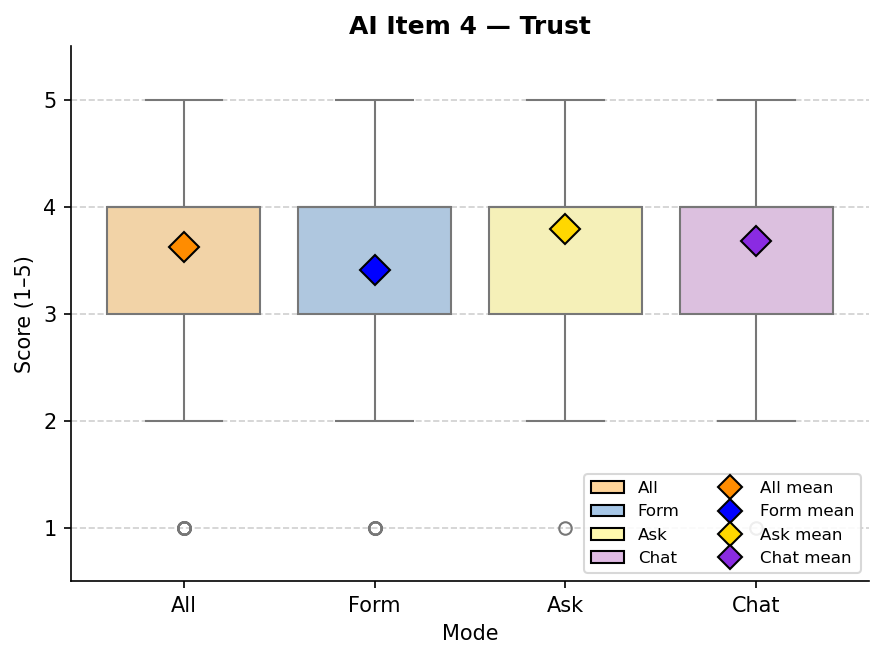
\includegraphics[width=0.88\linewidth,height=0.34\textheight,keepaspectratio]{ai_item_4_trust.png}
\end{column}
\begin{column}{0.5\textwidth}\centering
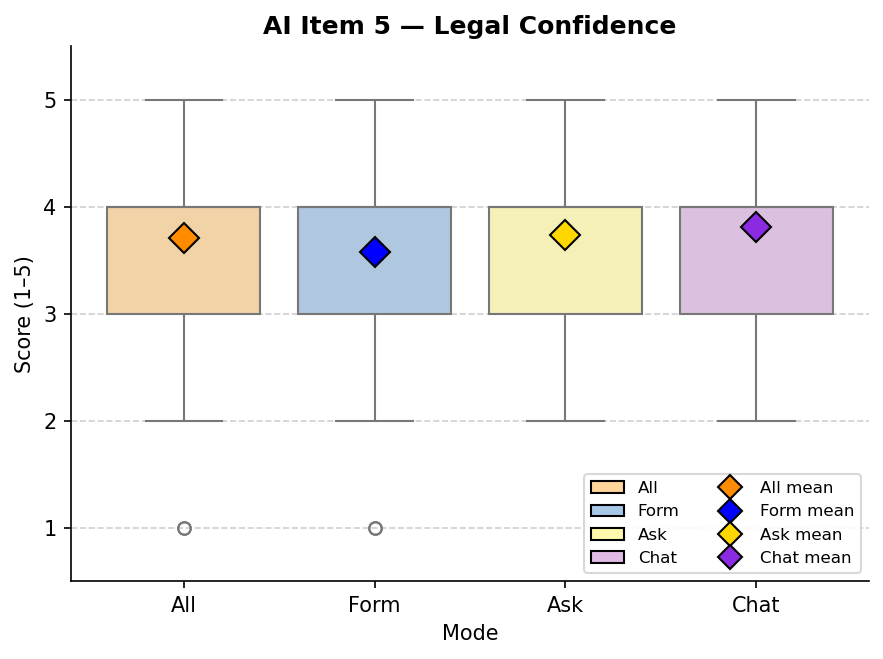
\includegraphics[width=0.88\linewidth,height=0.34\textheight,keepaspectratio]{ai_item_5_legal.png}
\end{column}
\end{columns}
\vspace{0.15cm}
\centering
\setlength{\tabcolsep}{16pt}\renewcommand{\arraystretch}{1.05}
\scriptsize
\begin{tabular}{@{}l ccc@{}}
\toprule
Metric & Form & Ask & Chat\\
\midrule
Completeness          & \textbf{4.84} & 3.84 & 3.18\\
Scenario Faithfulness & 1.84 & 2.30 & \textbf{2.49}\\
Legal Correctness     & \textbf{3.59} & 3.43 & 3.15\\
Hallucination (inverse) & 1.65 & 2.40 & \textbf{2.54}\\
Overall               & 2.41 & 2.49 & \textbf{2.62}\\
\bottomrule
\end{tabular}

\vspace{0.25cm}
\begin{minipage}{0.94\linewidth}\scriptsize\raggedright
By the judge, Form is worst on the holistic \emph{Overall} score while Chat is best,
but Chat leads \emph{only} there: on \textbf{Legal Correctness} (and perceived legal
confidence, Item~5) the ranking flips toward Form, suggesting the autonomous LLM can
read as \emph{too benign}, fluent yet less legally precise.
\par\vspace{0.1cm}{\color{uulmrule} Sources: Perceived AI Support (5-pt Likert);
LLM-as-a-Judge evaluation template~\cite{suJuDGEBenchmarkingJudgment2025}}
\end{minipage}
\end{frame}

% ============================================================
% 16-18 -- Mode screenshots revisited (RQ2/RQ3 quality angle)
% ============================================================
\begin{frame}{Form Mode -- Checkboxes}
\centering
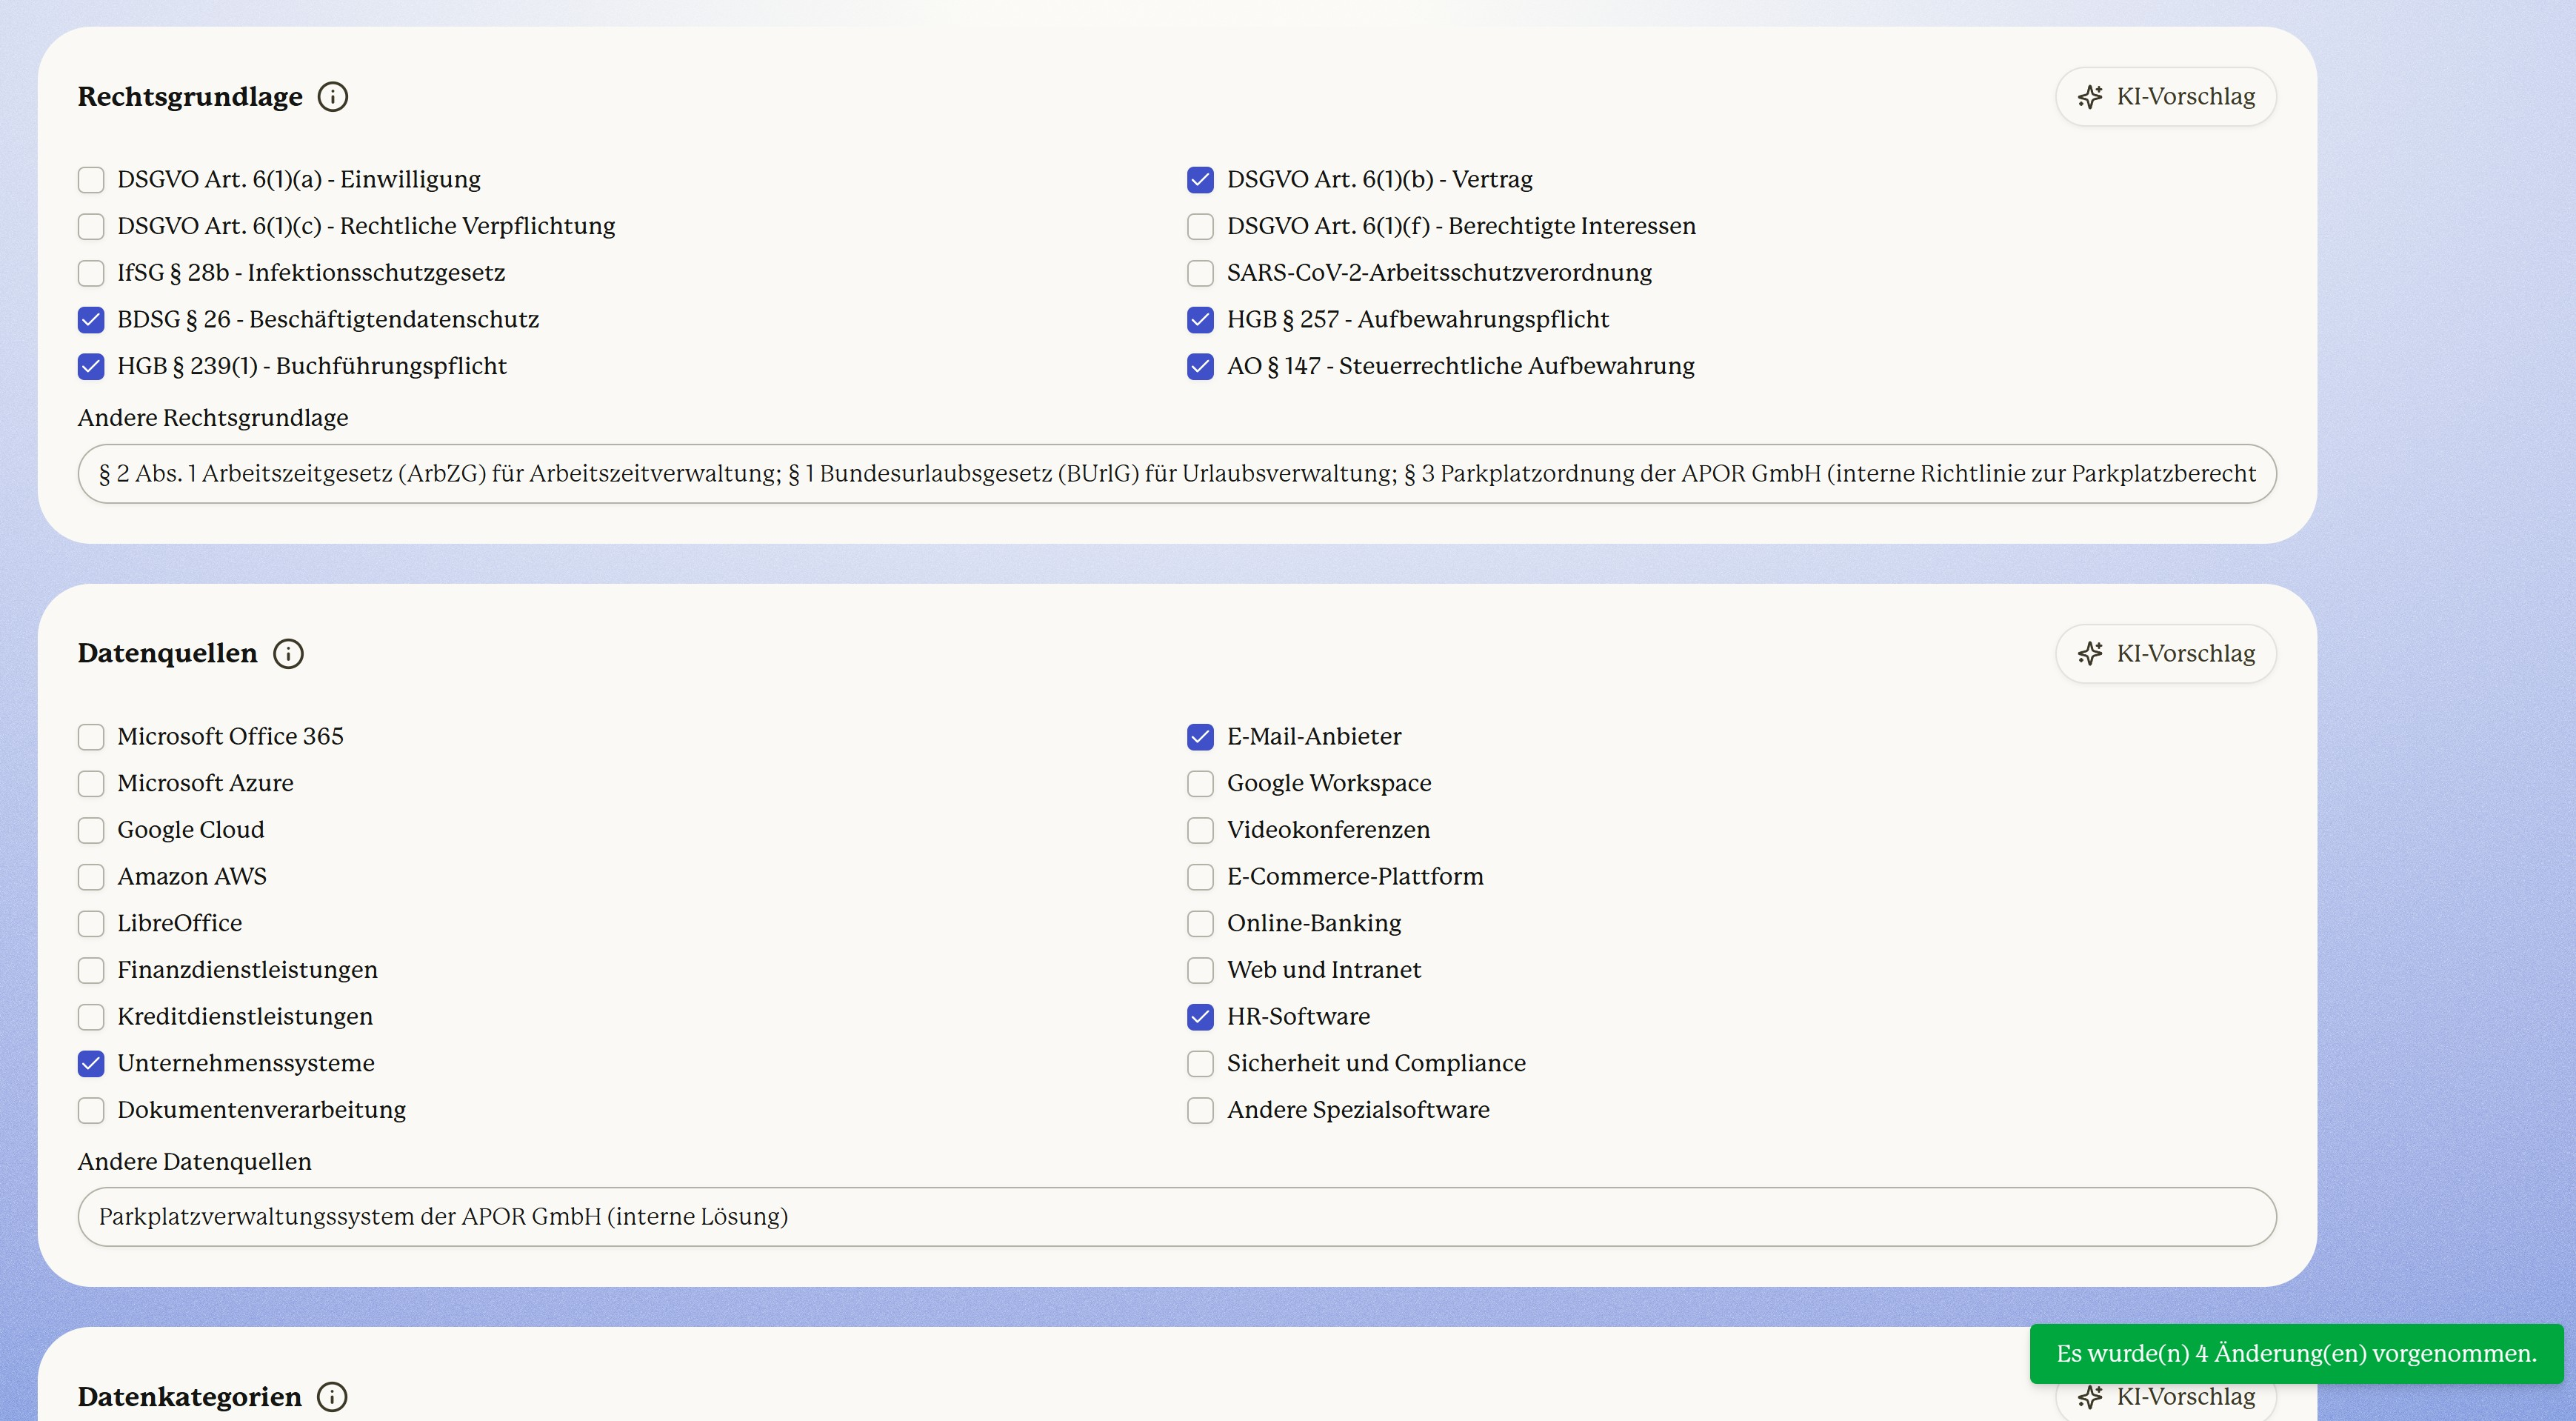
\includegraphics[width=0.92\linewidth,height=0.72\textheight,keepaspectratio]{ropagen-form.jpg}\\[0.15cm]
{\scriptsize \textbf{Entry point} for novices, but high recall comes with \textbf{overhead}: every required field is present, even content the user never actually described.}
\end{frame}

\begin{frame}{Ask Mode -- Hybrid}
\centering
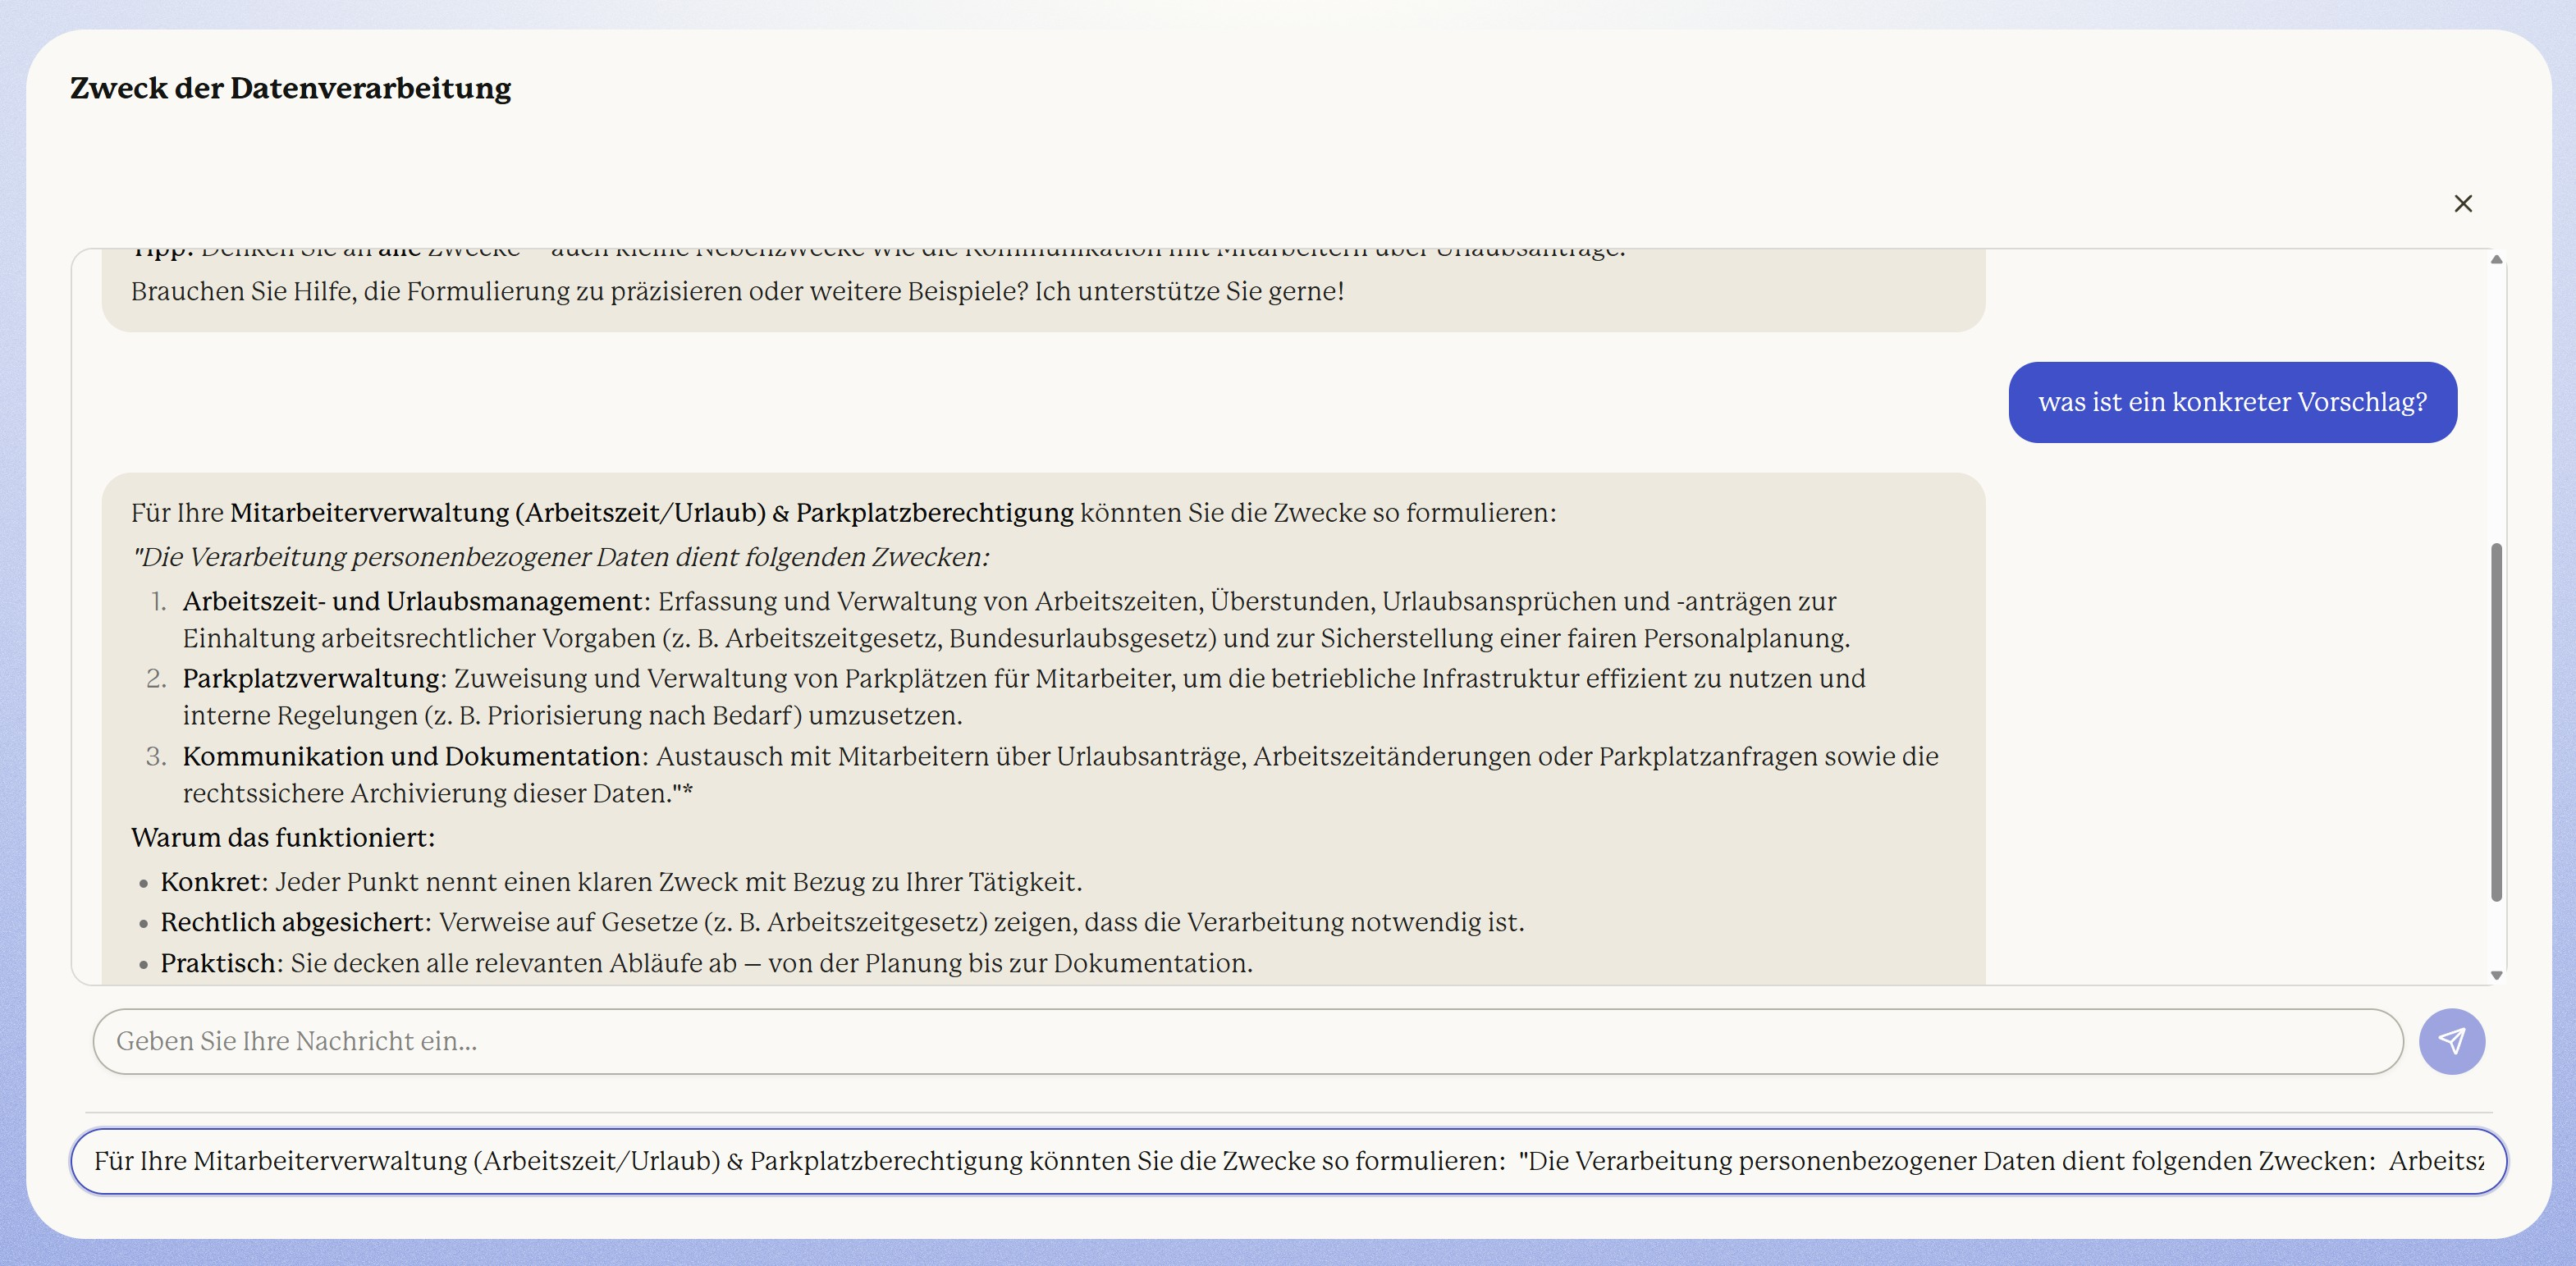
\includegraphics[width=0.92\linewidth,height=0.72\textheight,keepaspectratio]{ropagen-ask.jpg}\\[0.15cm]
{\scriptsize \textbf{Ask fails} the user it was built for: a novice cannot do everything alone (know what to ask). The LLM must act as a \textbf{co-author}, not wait to be asked.}
\end{frame}

\begin{frame}{Chat Mode -- Autonomous LLM}
\centering
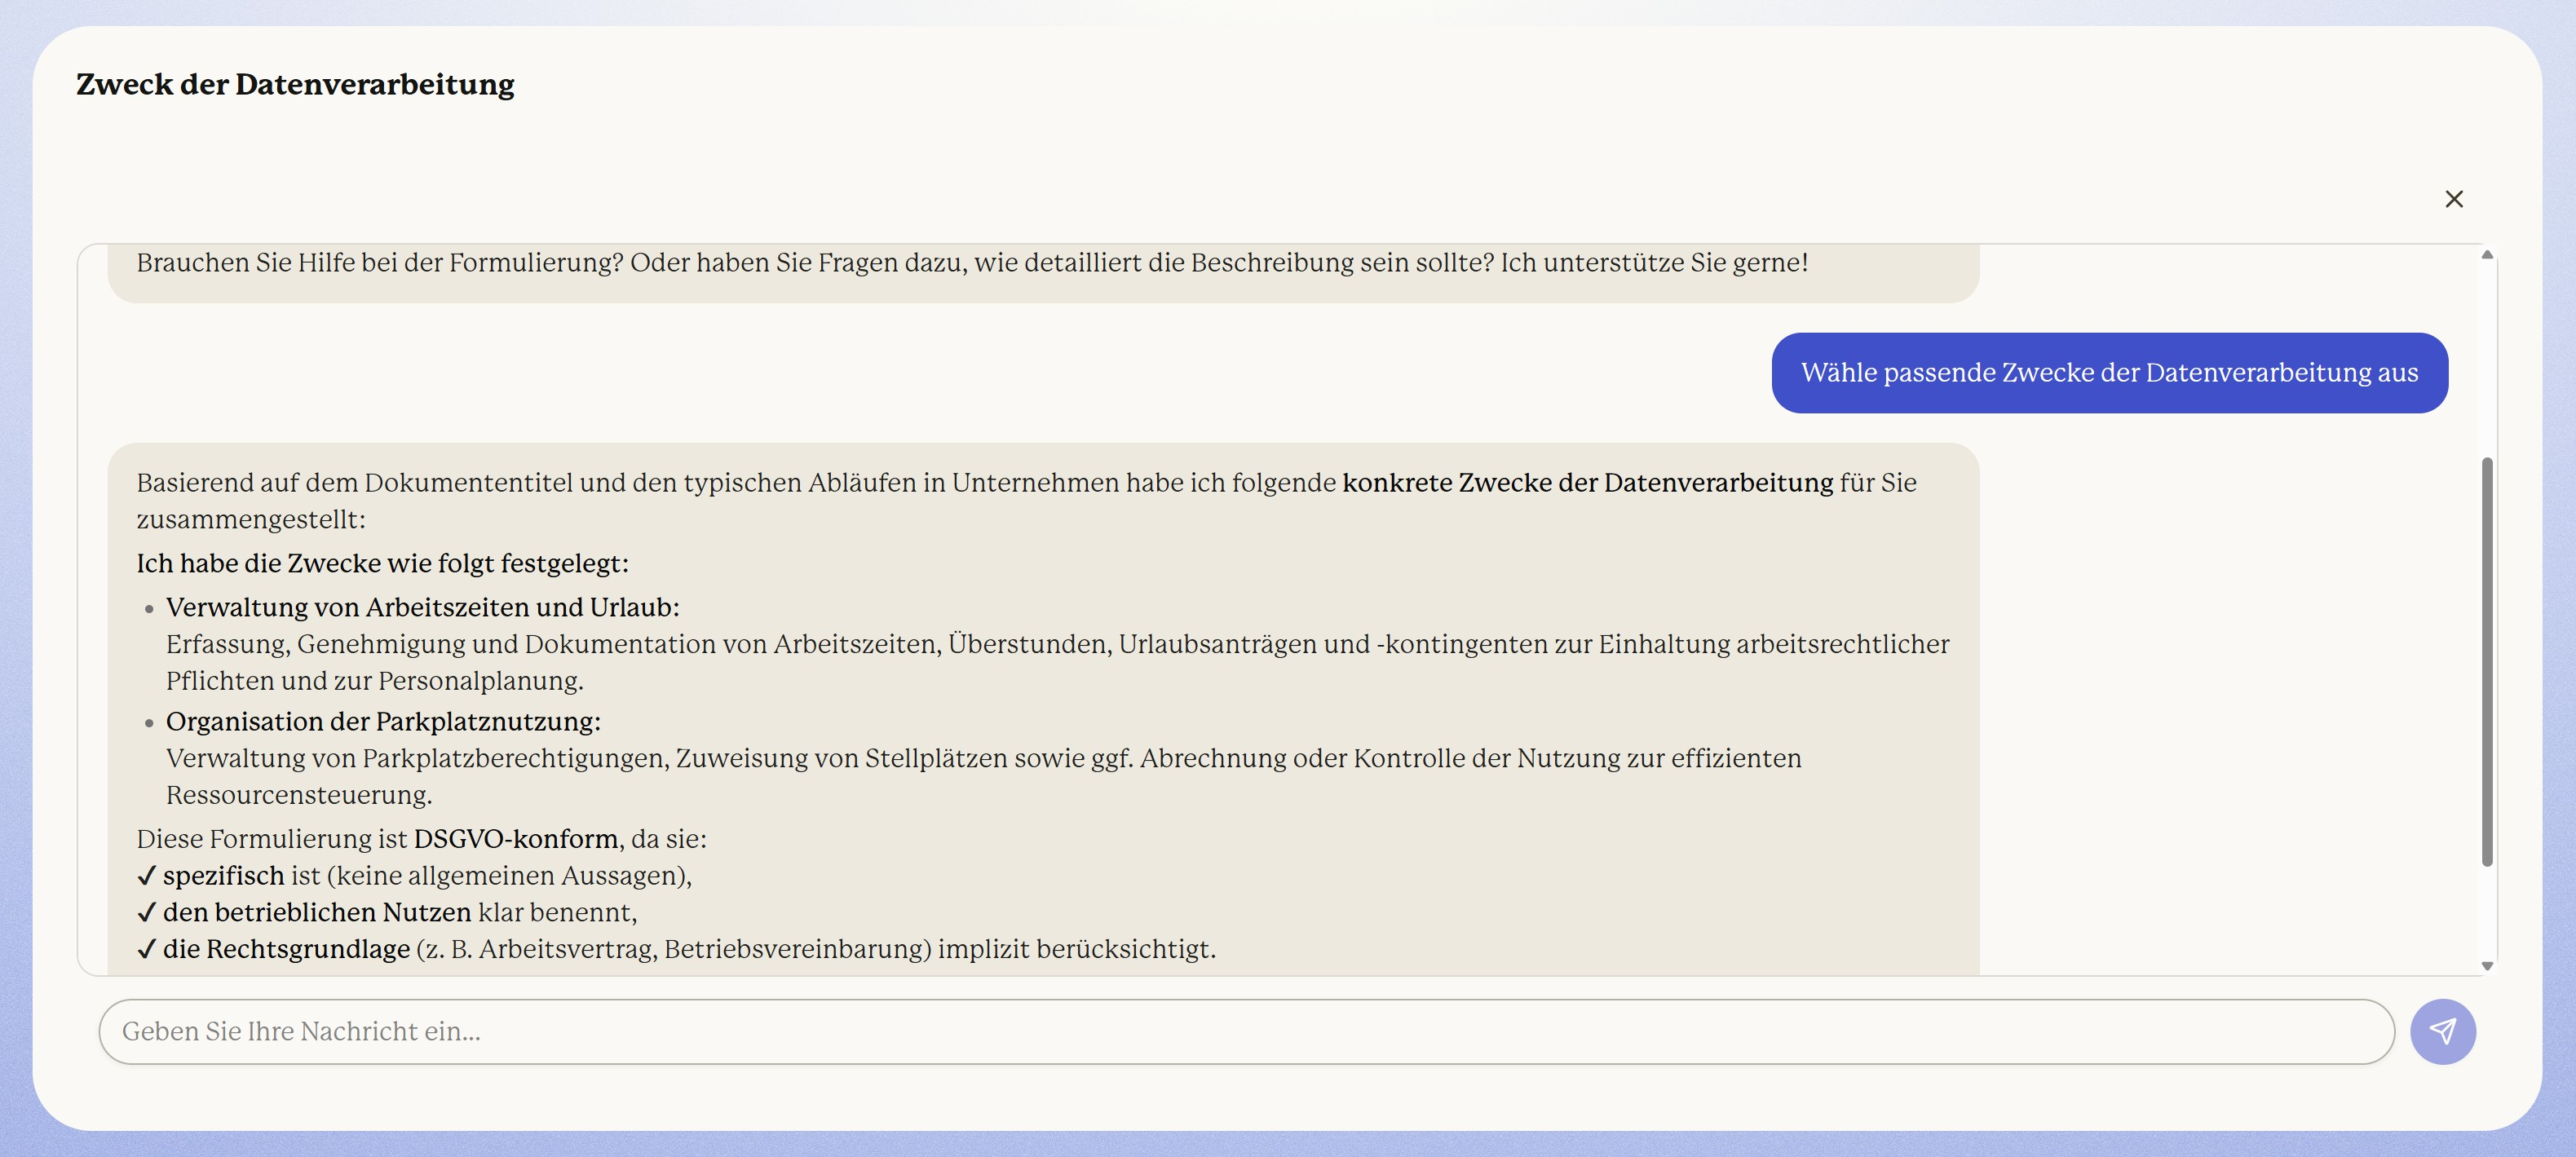
\includegraphics[width=0.92\linewidth,height=0.72\textheight,keepaspectratio]{ropagen-chat.jpg}\\[0.15cm]
{\scriptsize \textbf{Chat plays too much into the user} (it affirms rather than corrects) and trades completeness for grounding: \textbf{risk of omission}.}
\end{frame}

% ============================================================
% 19 -- Conclusion divider
% ============================================================
\begin{frame}
\redband{\centering{\fontsize{30}{34}\selectfont\bfseries Conclusion}}
\end{frame}

% ============================================================
% 19b -- Conclusion content (answers to the RQs)
% ============================================================
\begin{frame}{Conclusion}
\footnotesize
\linespread{0.96}\selectfont
\begin{itemize}
  \setlength{\itemsep}{0.13cm}
  \item \textbf{RQ1 --- Less support, not more, won the experience.} Form was the most usable,
        the lightest on cognitive load, the most preferred, and the fastest; four instruments
        converged. Ask lost structurally: a novice without GDPR knowledge does not know what to ask.
  \item \textbf{RQ2 --- Each mode trades one risk for another.} Form supports \emph{inclusion}
        (every required field present, though some was never described by the user); Chat supports
        \emph{precision} (grounded in the scenario, though content may be missing); Ask trails both.
        An incomplete ROPA is the worse legal risk; a complete-but-fabricated one the worse operational risk.
  \item \textbf{RQ3 --- Confidence does not track quality.} Users felt most confident in the
        conversational modes, yet on legal correctness the judge rated those lowest; conversational
        LLMs default to affirming the user's framing.
  \item \textbf{Contribution --- a content-typed assignment.} \emph{Enumerable} sub-records (e.g.
        legal bases under Art~6(1)) belong in a checkbox UI; \emph{scenario-specific} sub-records
        (e.g. retention periods, technical \& organizational measures) belong in conversational
        extraction. Legal-vocabulary quality is model-side, not UI-side. Form can also serve as a
        novice's \textbf{entry point}, a scaffold from which to build GDPR expertise before moving
        to freer interaction.
  \item \textbf{Takeaway --- redistribution, not replacement.} The LLM is a co-author, not a
        teacher: neither a novice nor a model alone produces a valid ROPA; the Article~30 document
        exists only where the two meet.
\end{itemize}
\end{frame}

% ============================================================
% 19c -- Limitations
% ============================================================
\begin{frame}{Limitations}
\footnotesize
\linespread{0.97}\selectfont
\begin{itemize}
  \setlength{\itemsep}{0.22cm}
  \item \textbf{Breadth over depth.} The cross-stream design was needed to compare confidence
        against quality (RQ3), but no single thread reached full depth: Ask's mechanism and the
        chapter-level NLP patterns could each support a study of their own.
  \item \textbf{Sample profile.} Participants were \textbf{IT-leaning, chatbot-fluent students}
        (majority male, mid-twenties). Older, non-IT staff who actually own ROPA documentation may
        calibrate confidence and quality differently, and may favor Chat less than this sample did.
  \item \textbf{Prototype tool, fixed model.} ROPAgen is a research prototype on a single
        \textbf{2025 Mistral} checkpoint shared by all modes. Relative mode trade-offs should
        survive a model swap (they rest on the interaction surface), but the \emph{absolute}
        quality figures are tied to this checkpoint and should not be extrapolated.
  \item \textbf{Evaluation instruments.} A \textbf{single} expert reference (checkbox-derived,
        slightly favoring Form on coverage) and a \textbf{single-pass LLM-as-judge} without
        inter-rater replication or legal-expert validation. Multi-reference scoring and a
        multi-model judge ensemble would strengthen both layers.
  \item \textbf{Quality ceiling.} No mode reached the rubric midpoint on the Overall score, so
        the ceiling on document quality cannot be raised by interaction redesign alone.
\end{itemize}
\end{frame}

% ============================================================
% 20 -- Detailed Data Plots divider (backup)
% ============================================================
\begin{frame}
\redband{\centering{\fontsize{30}{34}\selectfont\bfseries Detailed Data Plots}}
\end{frame}

% ============================================================
% 21-26 -- Backup detail plots
% ============================================================
\begin{frame}{SUS Detail}
\centering
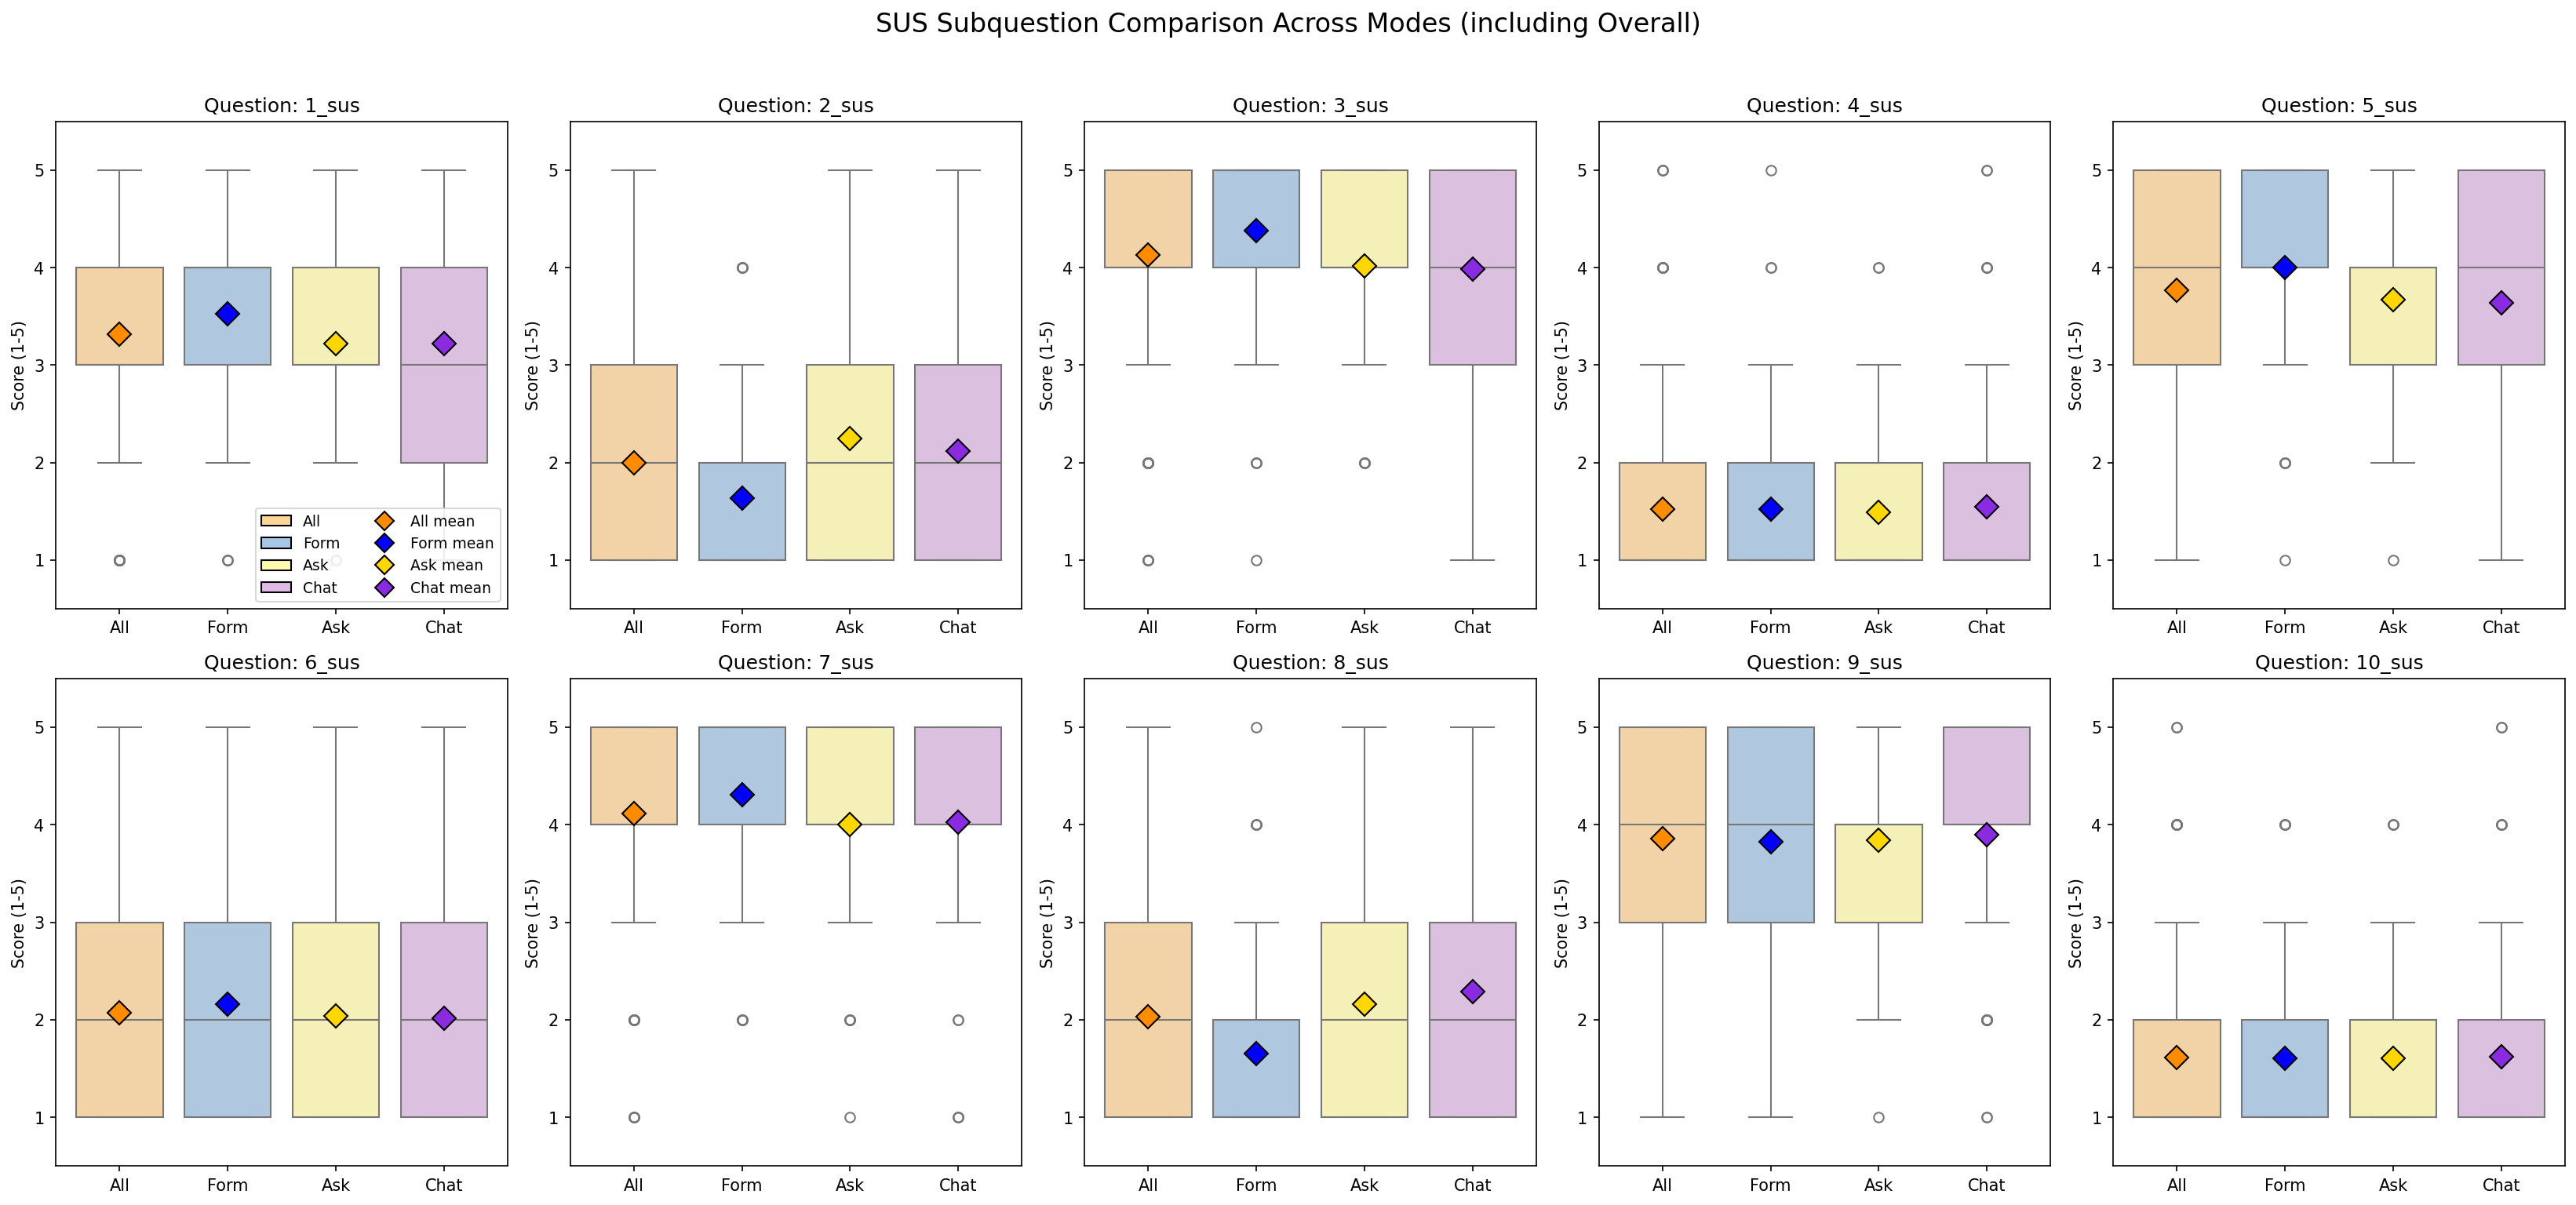
\includegraphics[width=\linewidth,height=0.80\textheight,keepaspectratio]{sus_subquestions_boxplot.png}
\end{frame}

\begin{frame}{NASA R-TLX Detail}
\centering
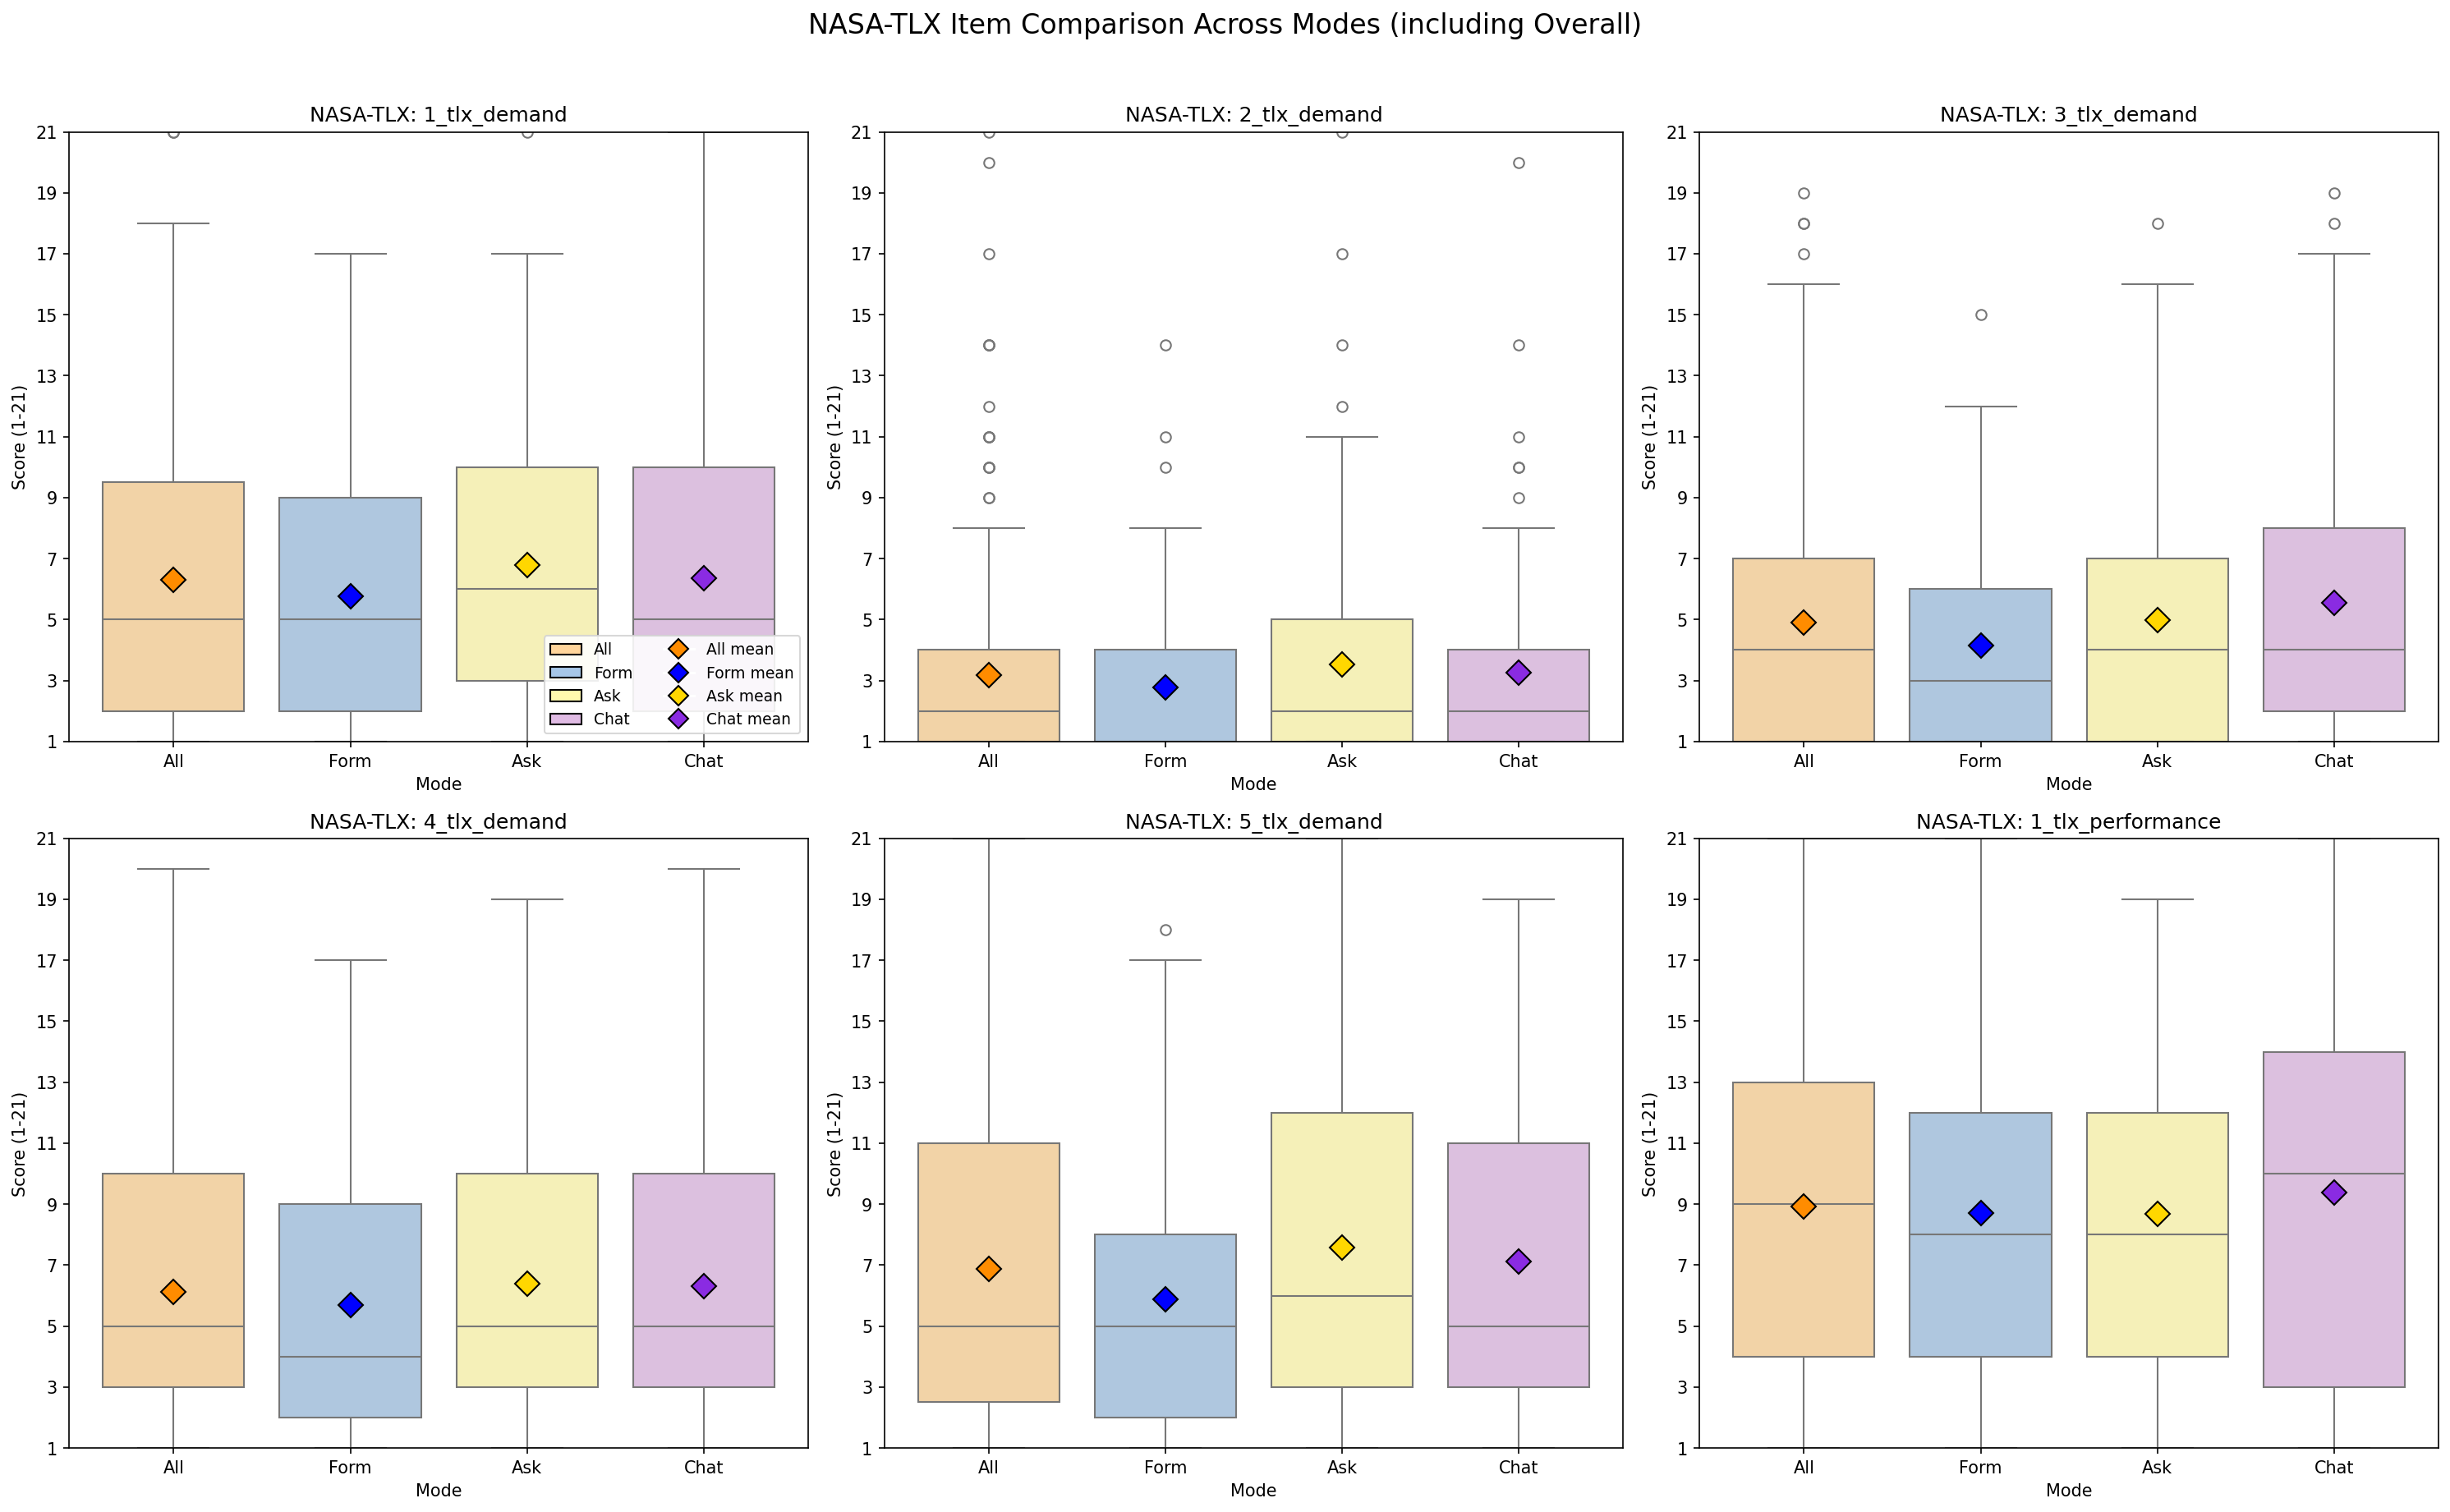
\includegraphics[width=\linewidth,height=0.80\textheight,keepaspectratio]{tlx_subquestions_boxplot.png}
\end{frame}

\begin{frame}{NLP Metrics (Document)}
\centering
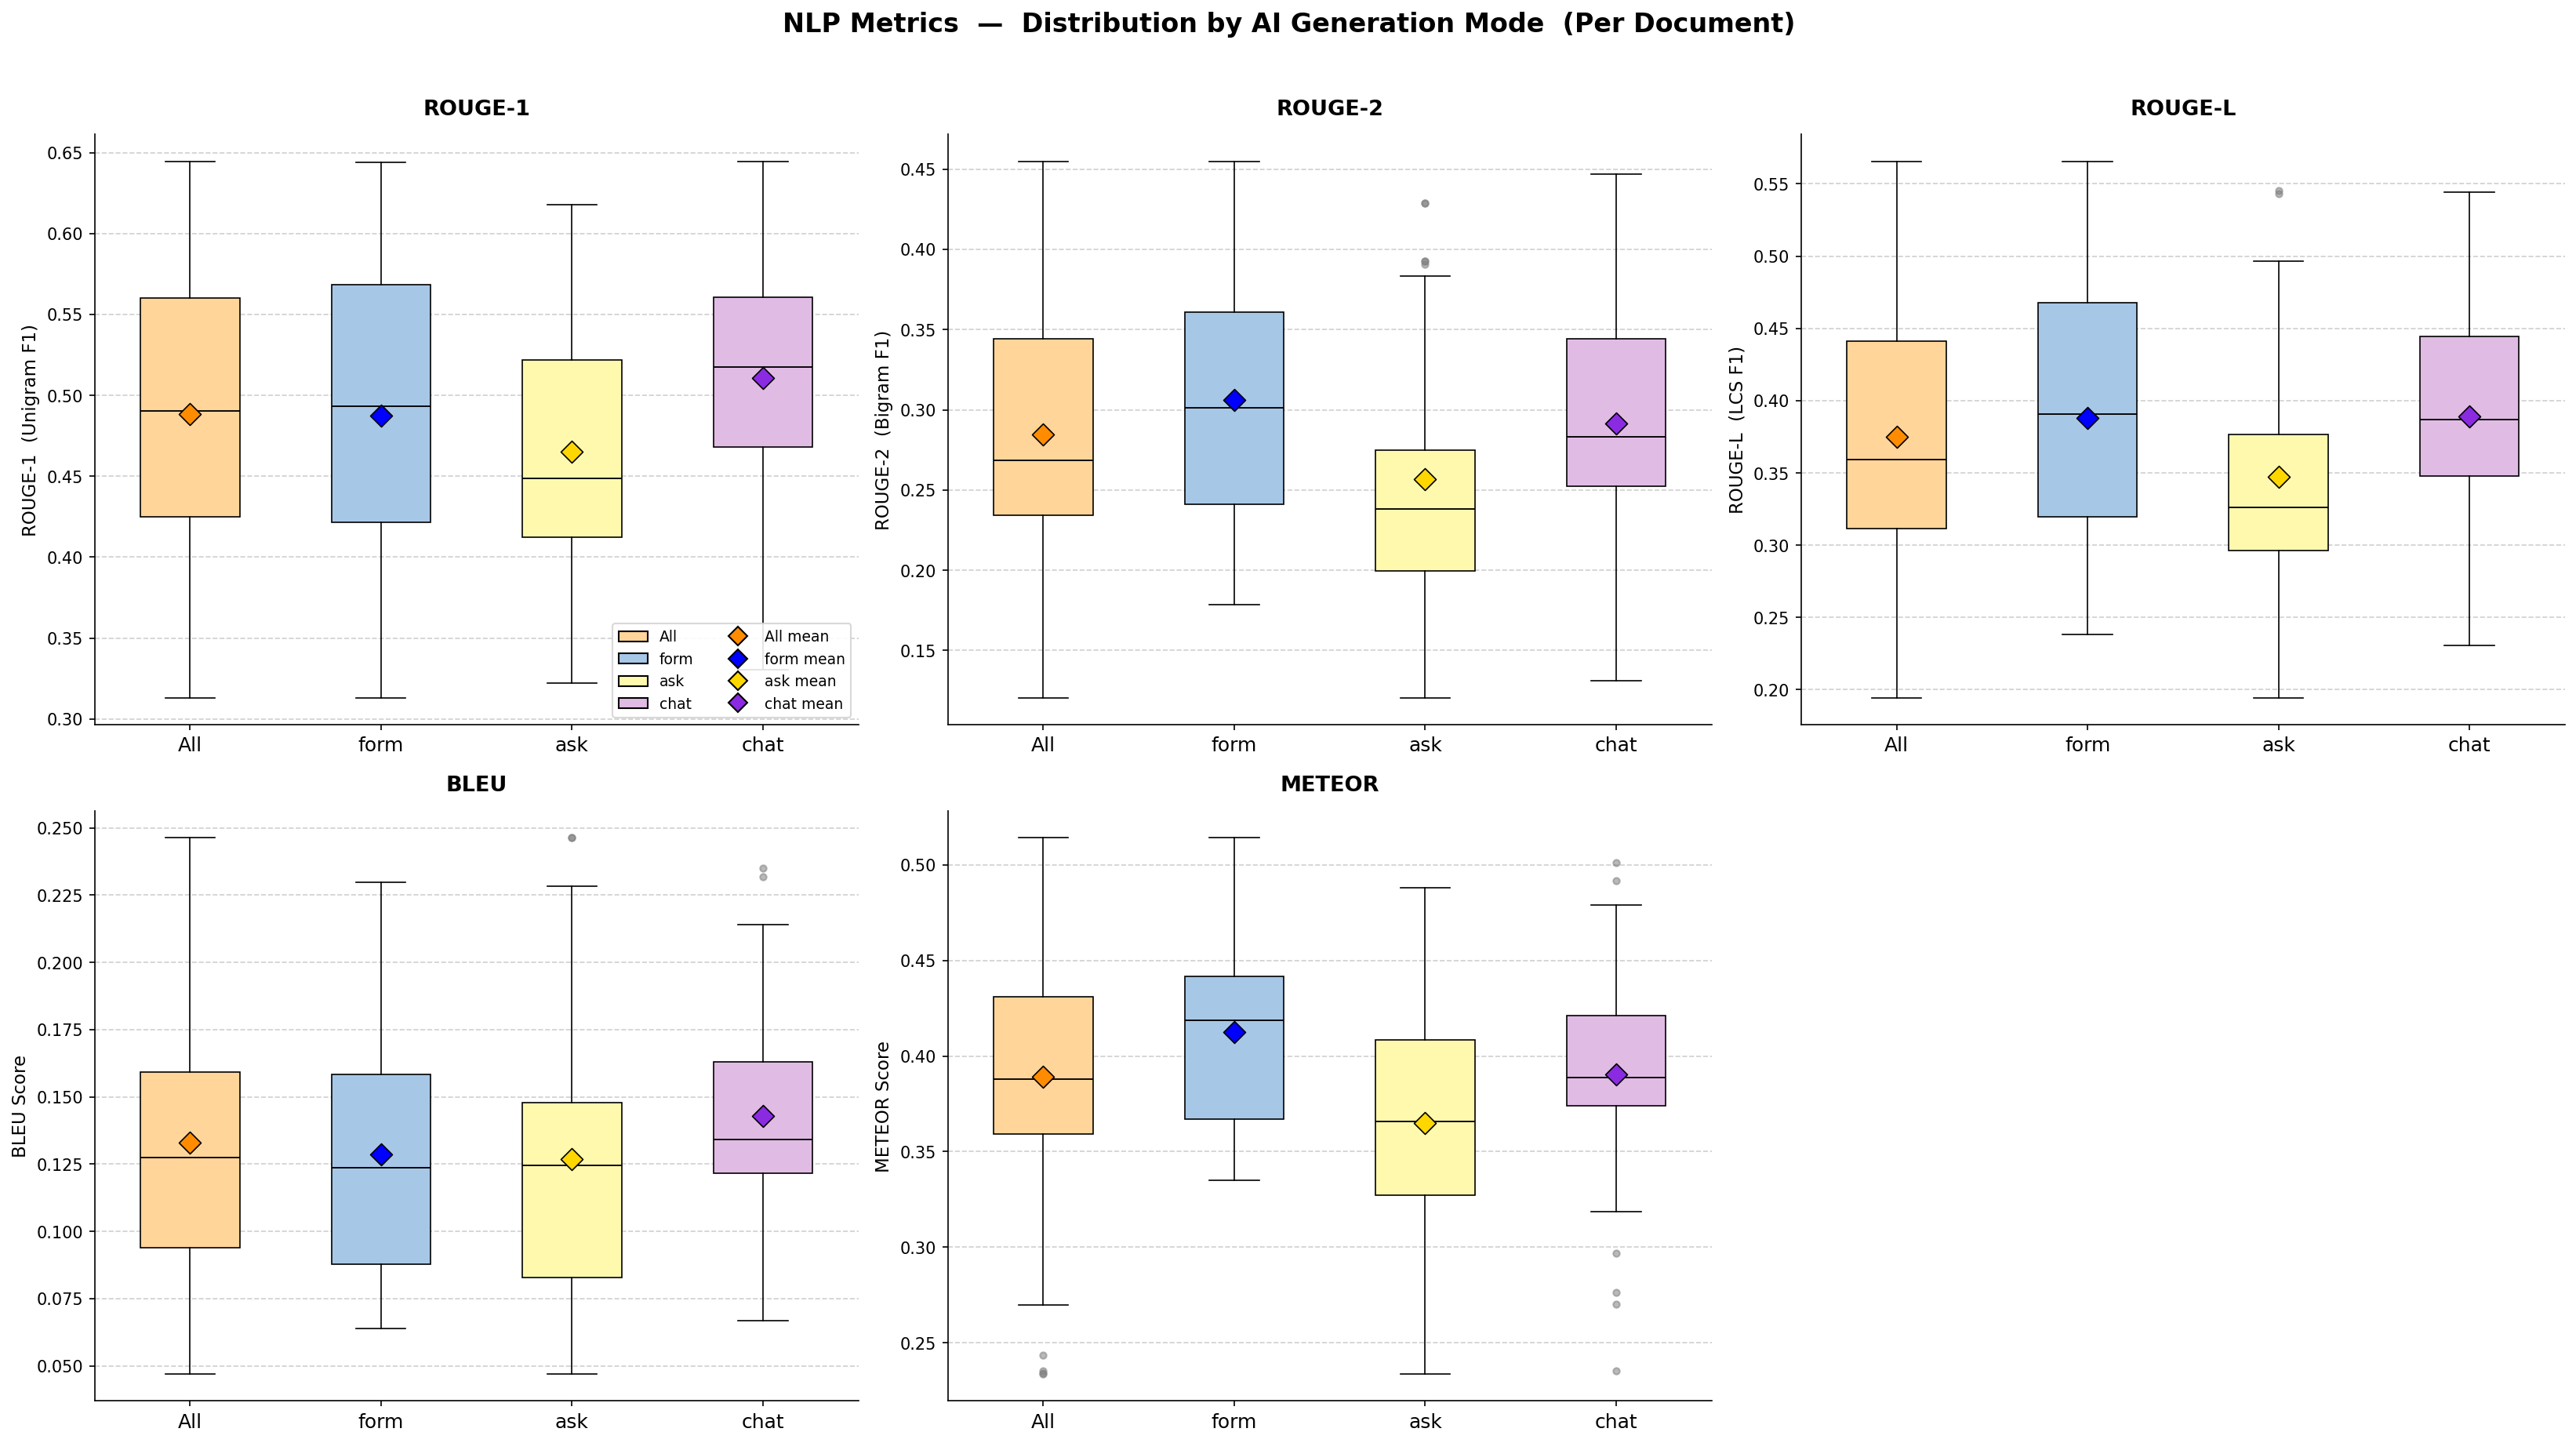
\includegraphics[width=\linewidth,height=0.80\textheight,keepaspectratio]{nlp_metrics_boxplot.png}
\end{frame}

\begin{frame}{BERT Metrics (Document)}
\centering
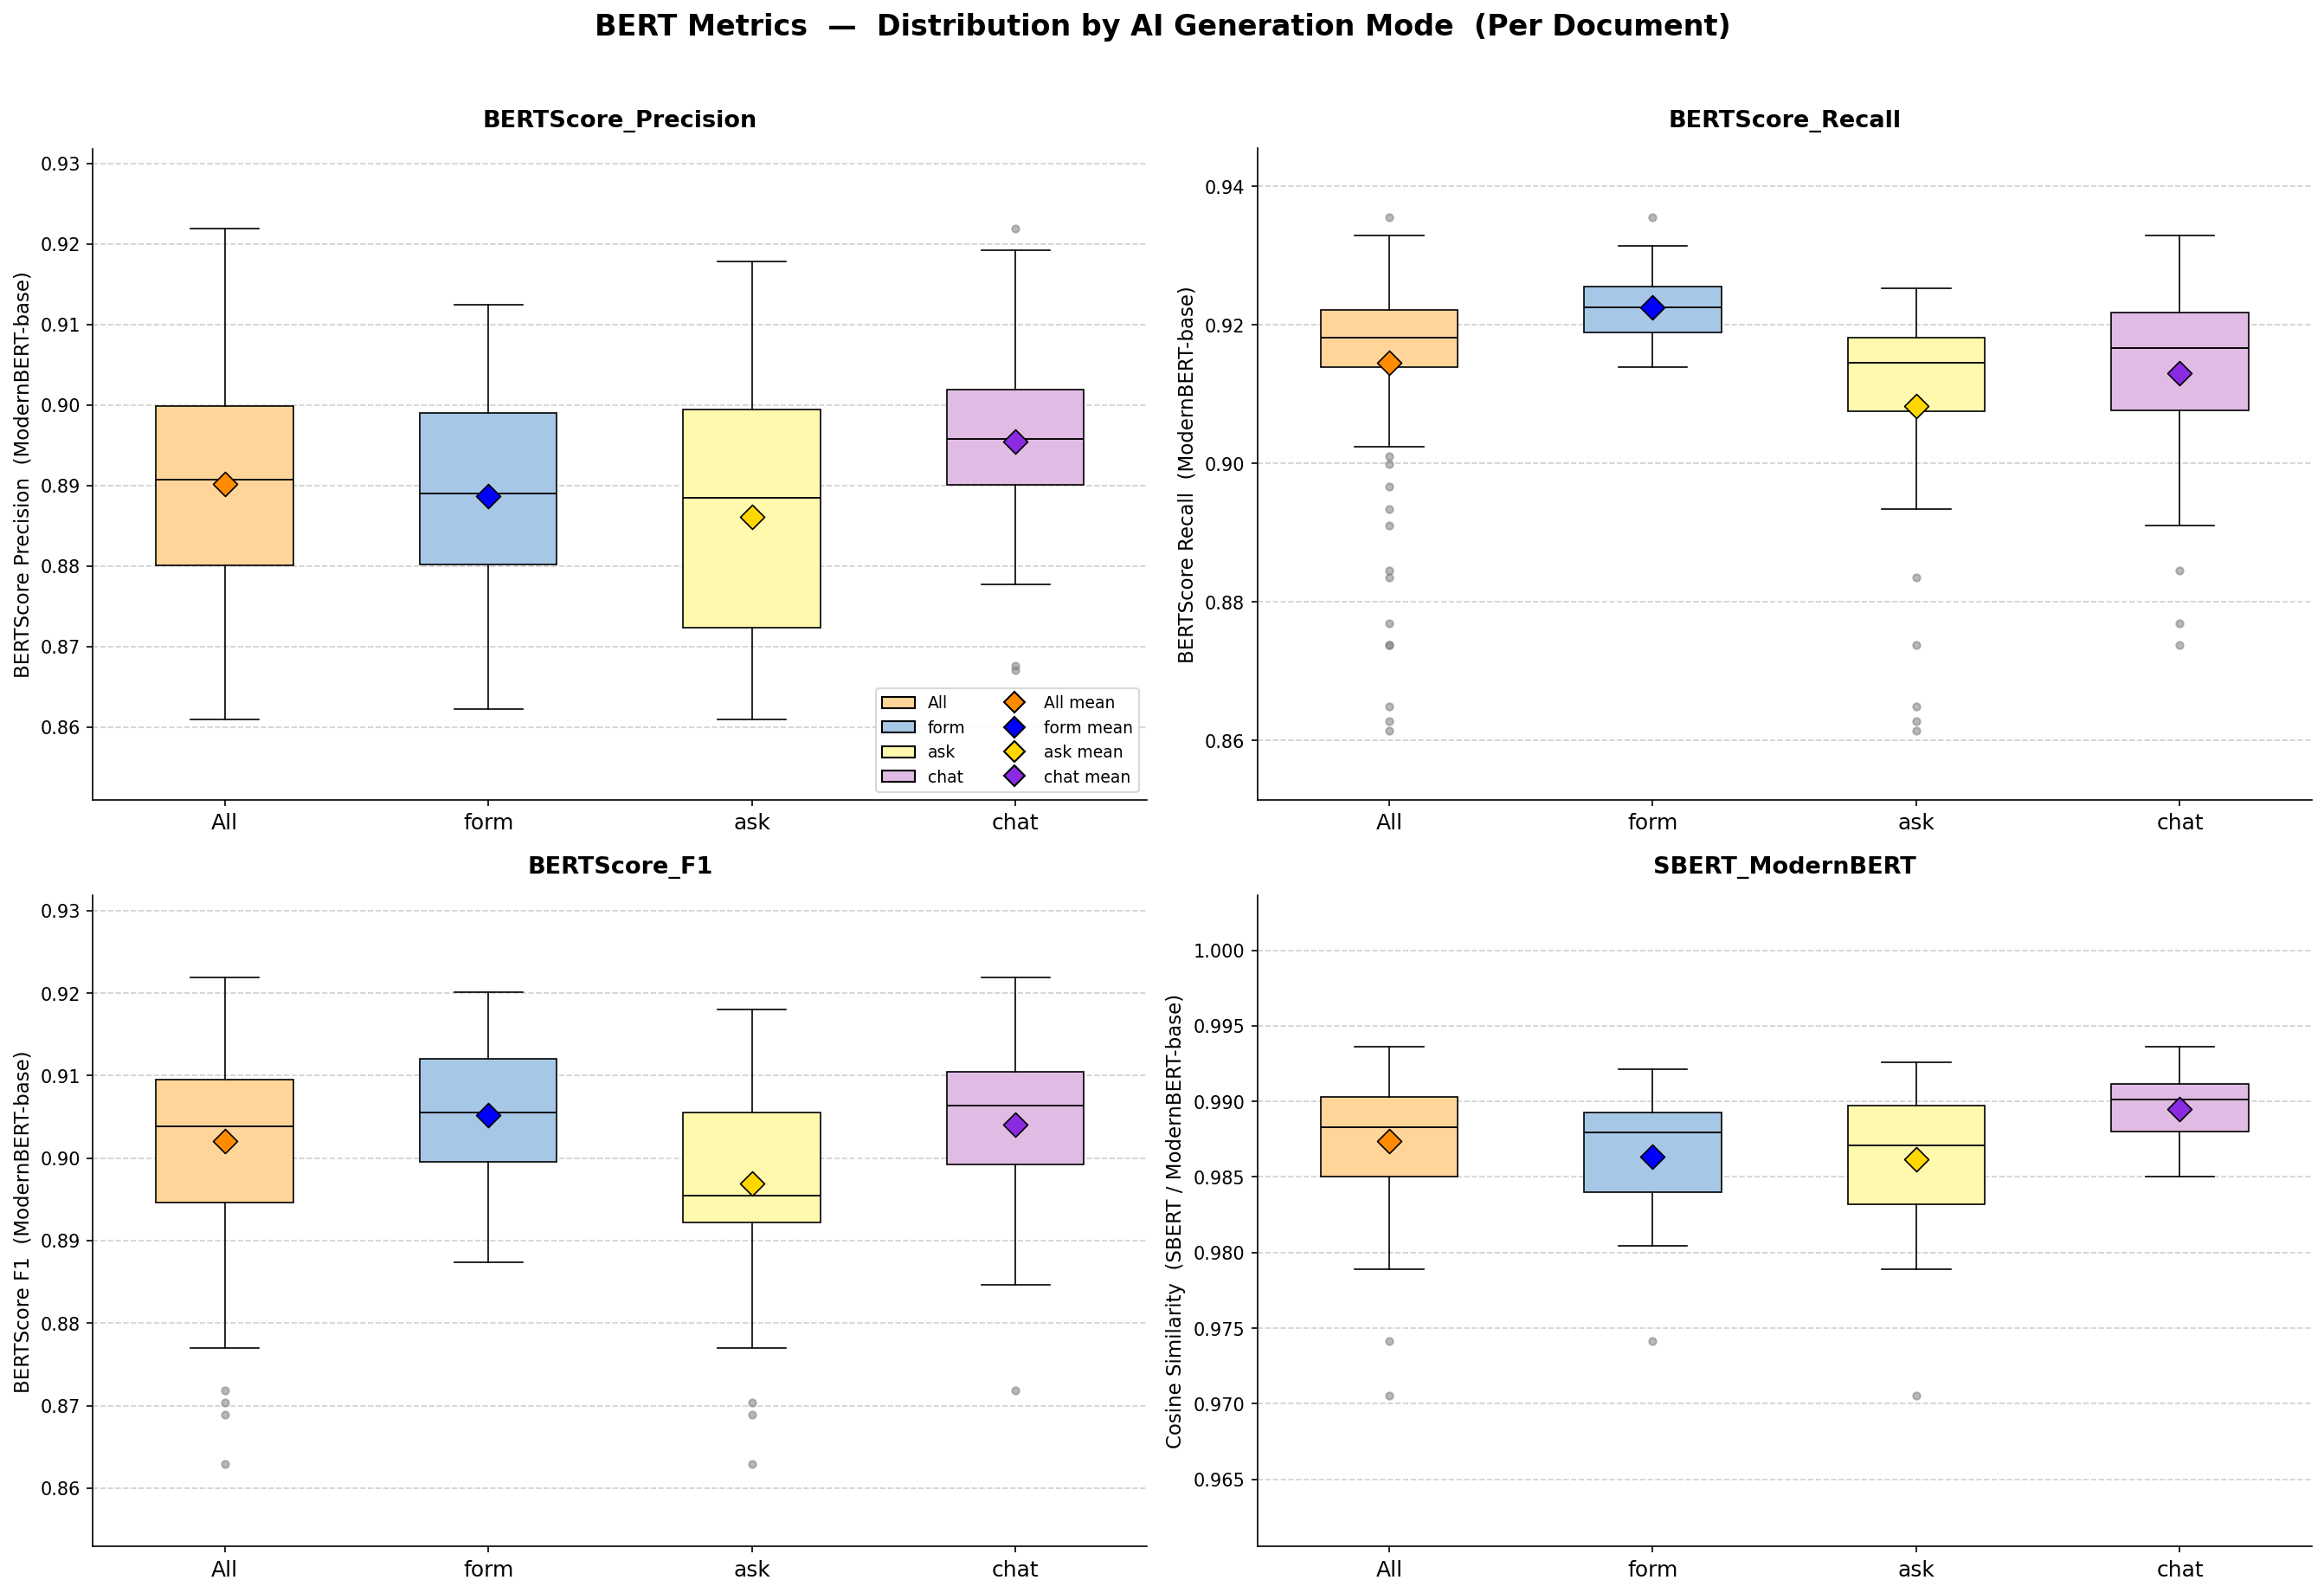
\includegraphics[width=\linewidth,height=0.80\textheight,keepaspectratio]{bert_metrics_boxplot.png}
\end{frame}

\begin{frame}{NLP Metrics (Chapter)}
\centering
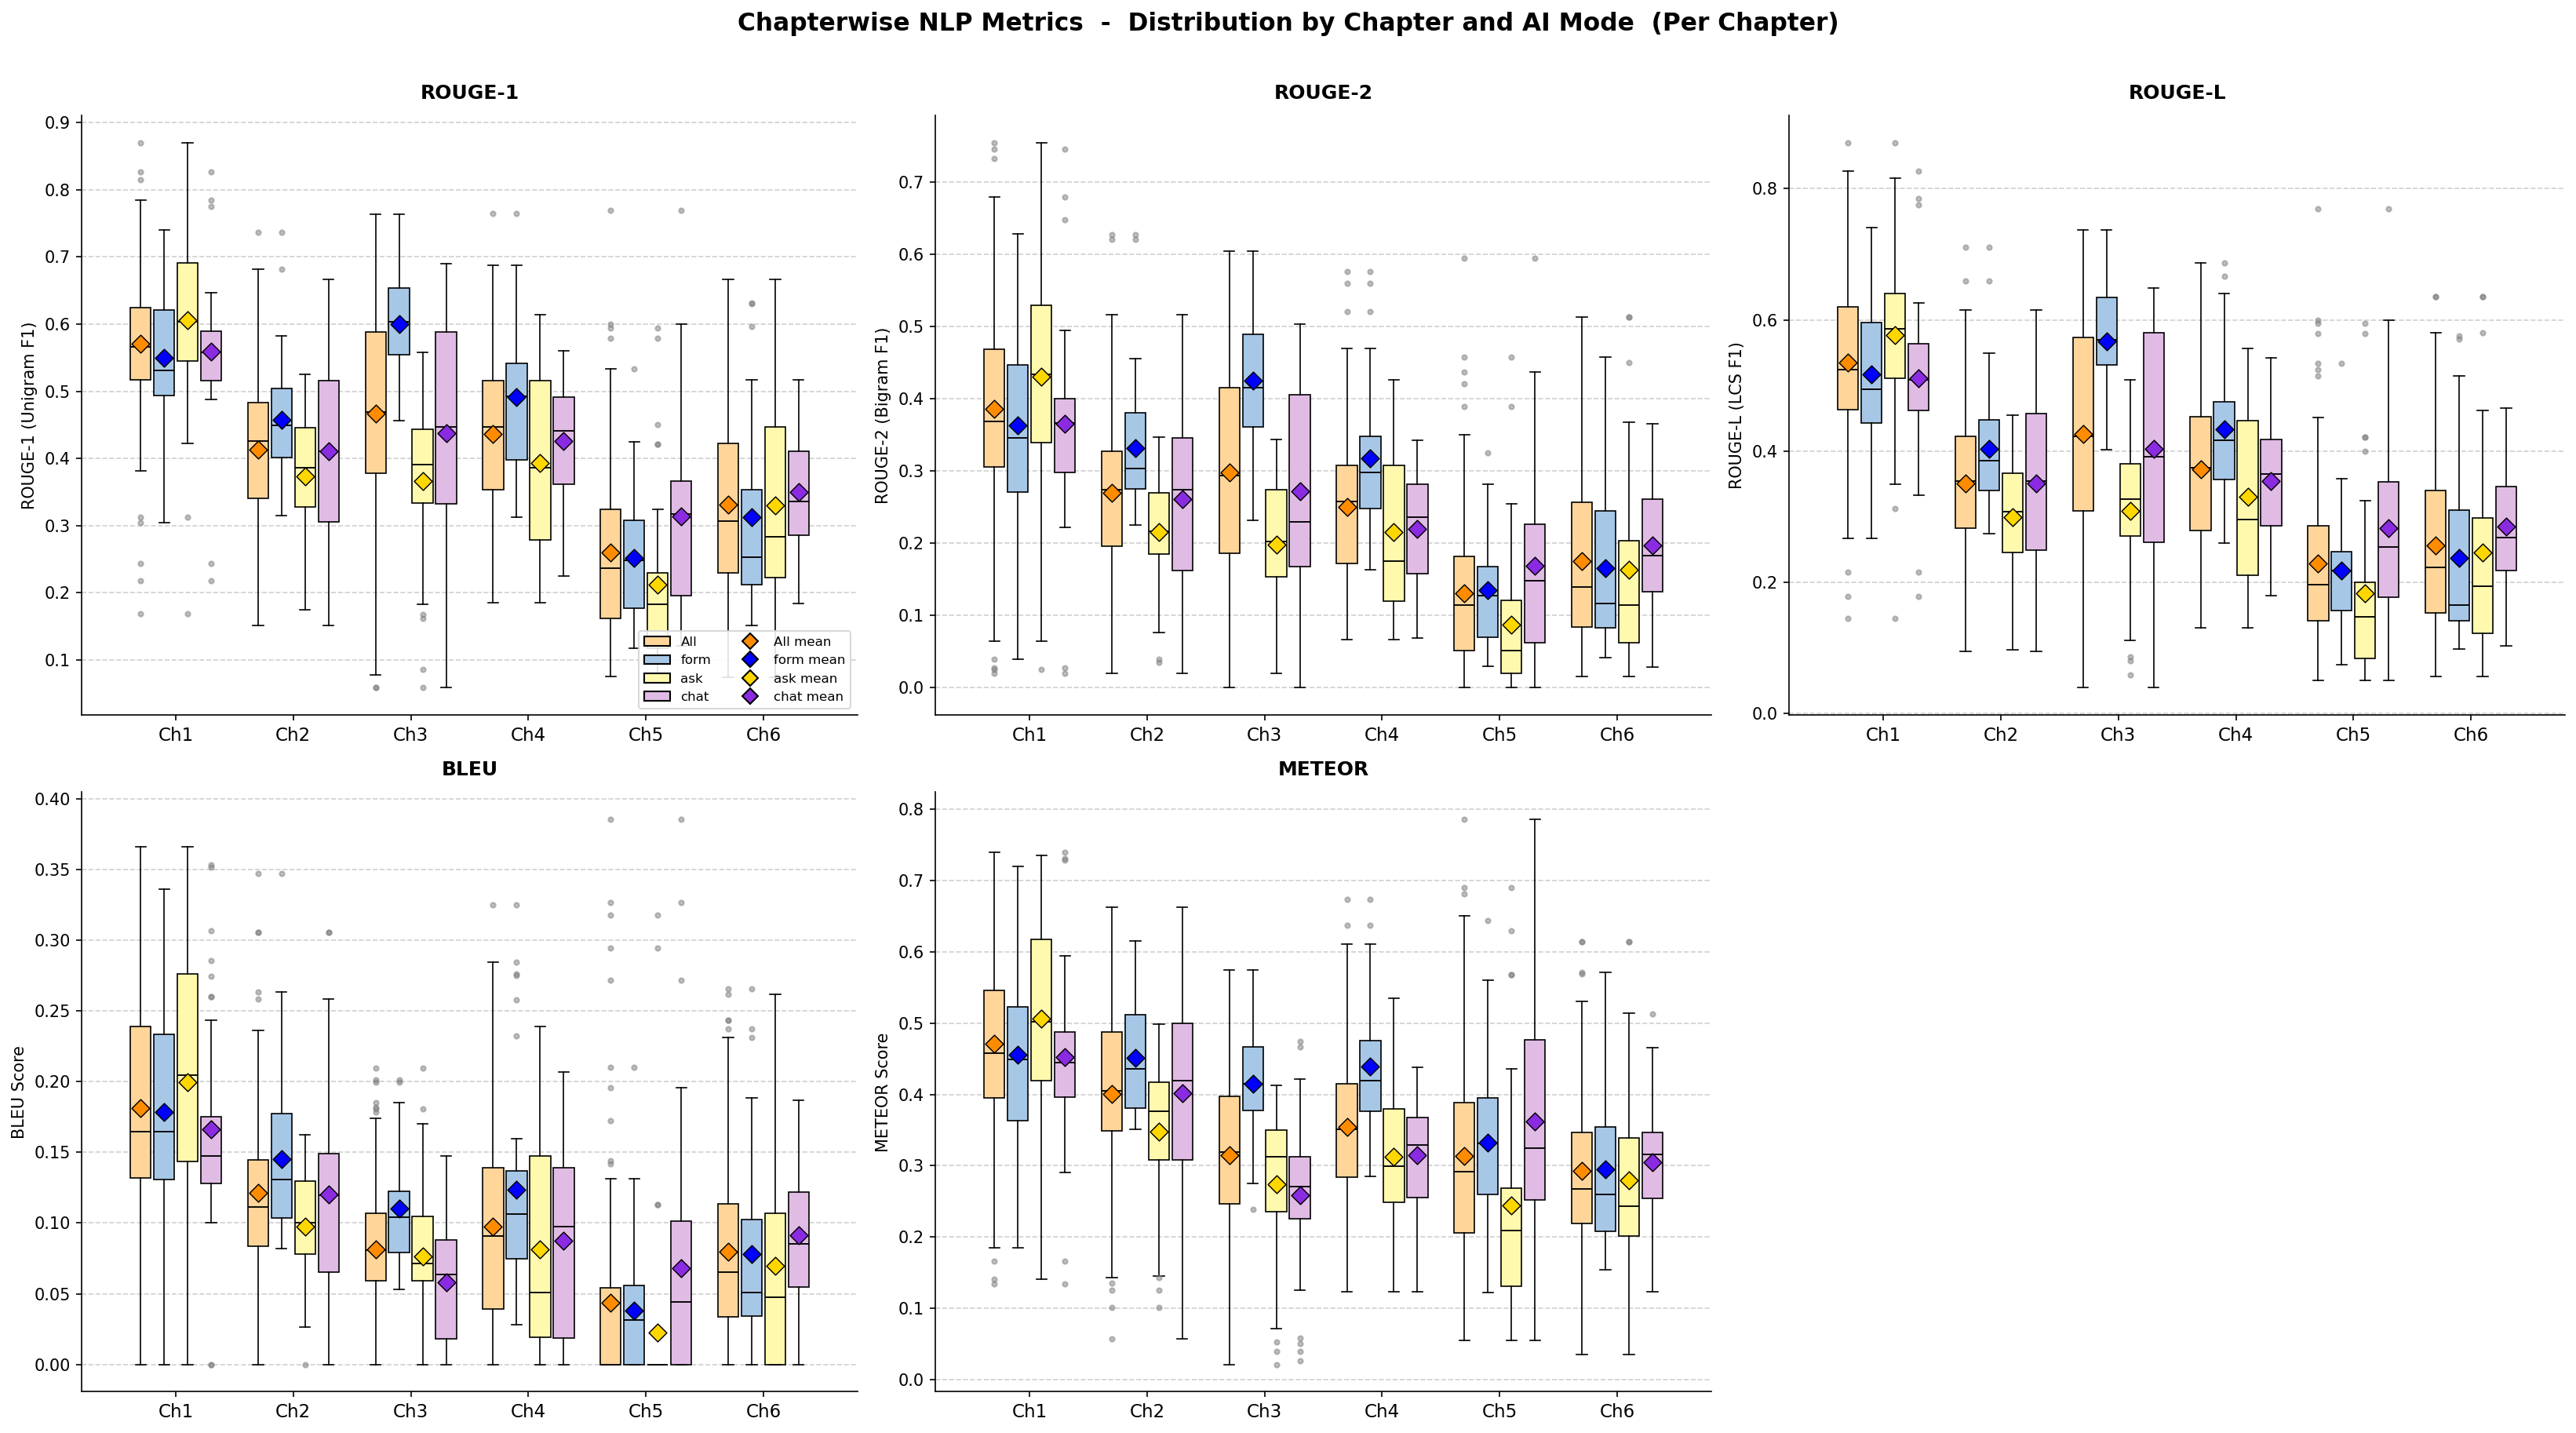
\includegraphics[width=\linewidth,height=0.80\textheight,keepaspectratio]{chapter_nlp_metrics_boxplot.png}
\end{frame}

\begin{frame}{BERT Metrics (Chapter)}
\centering
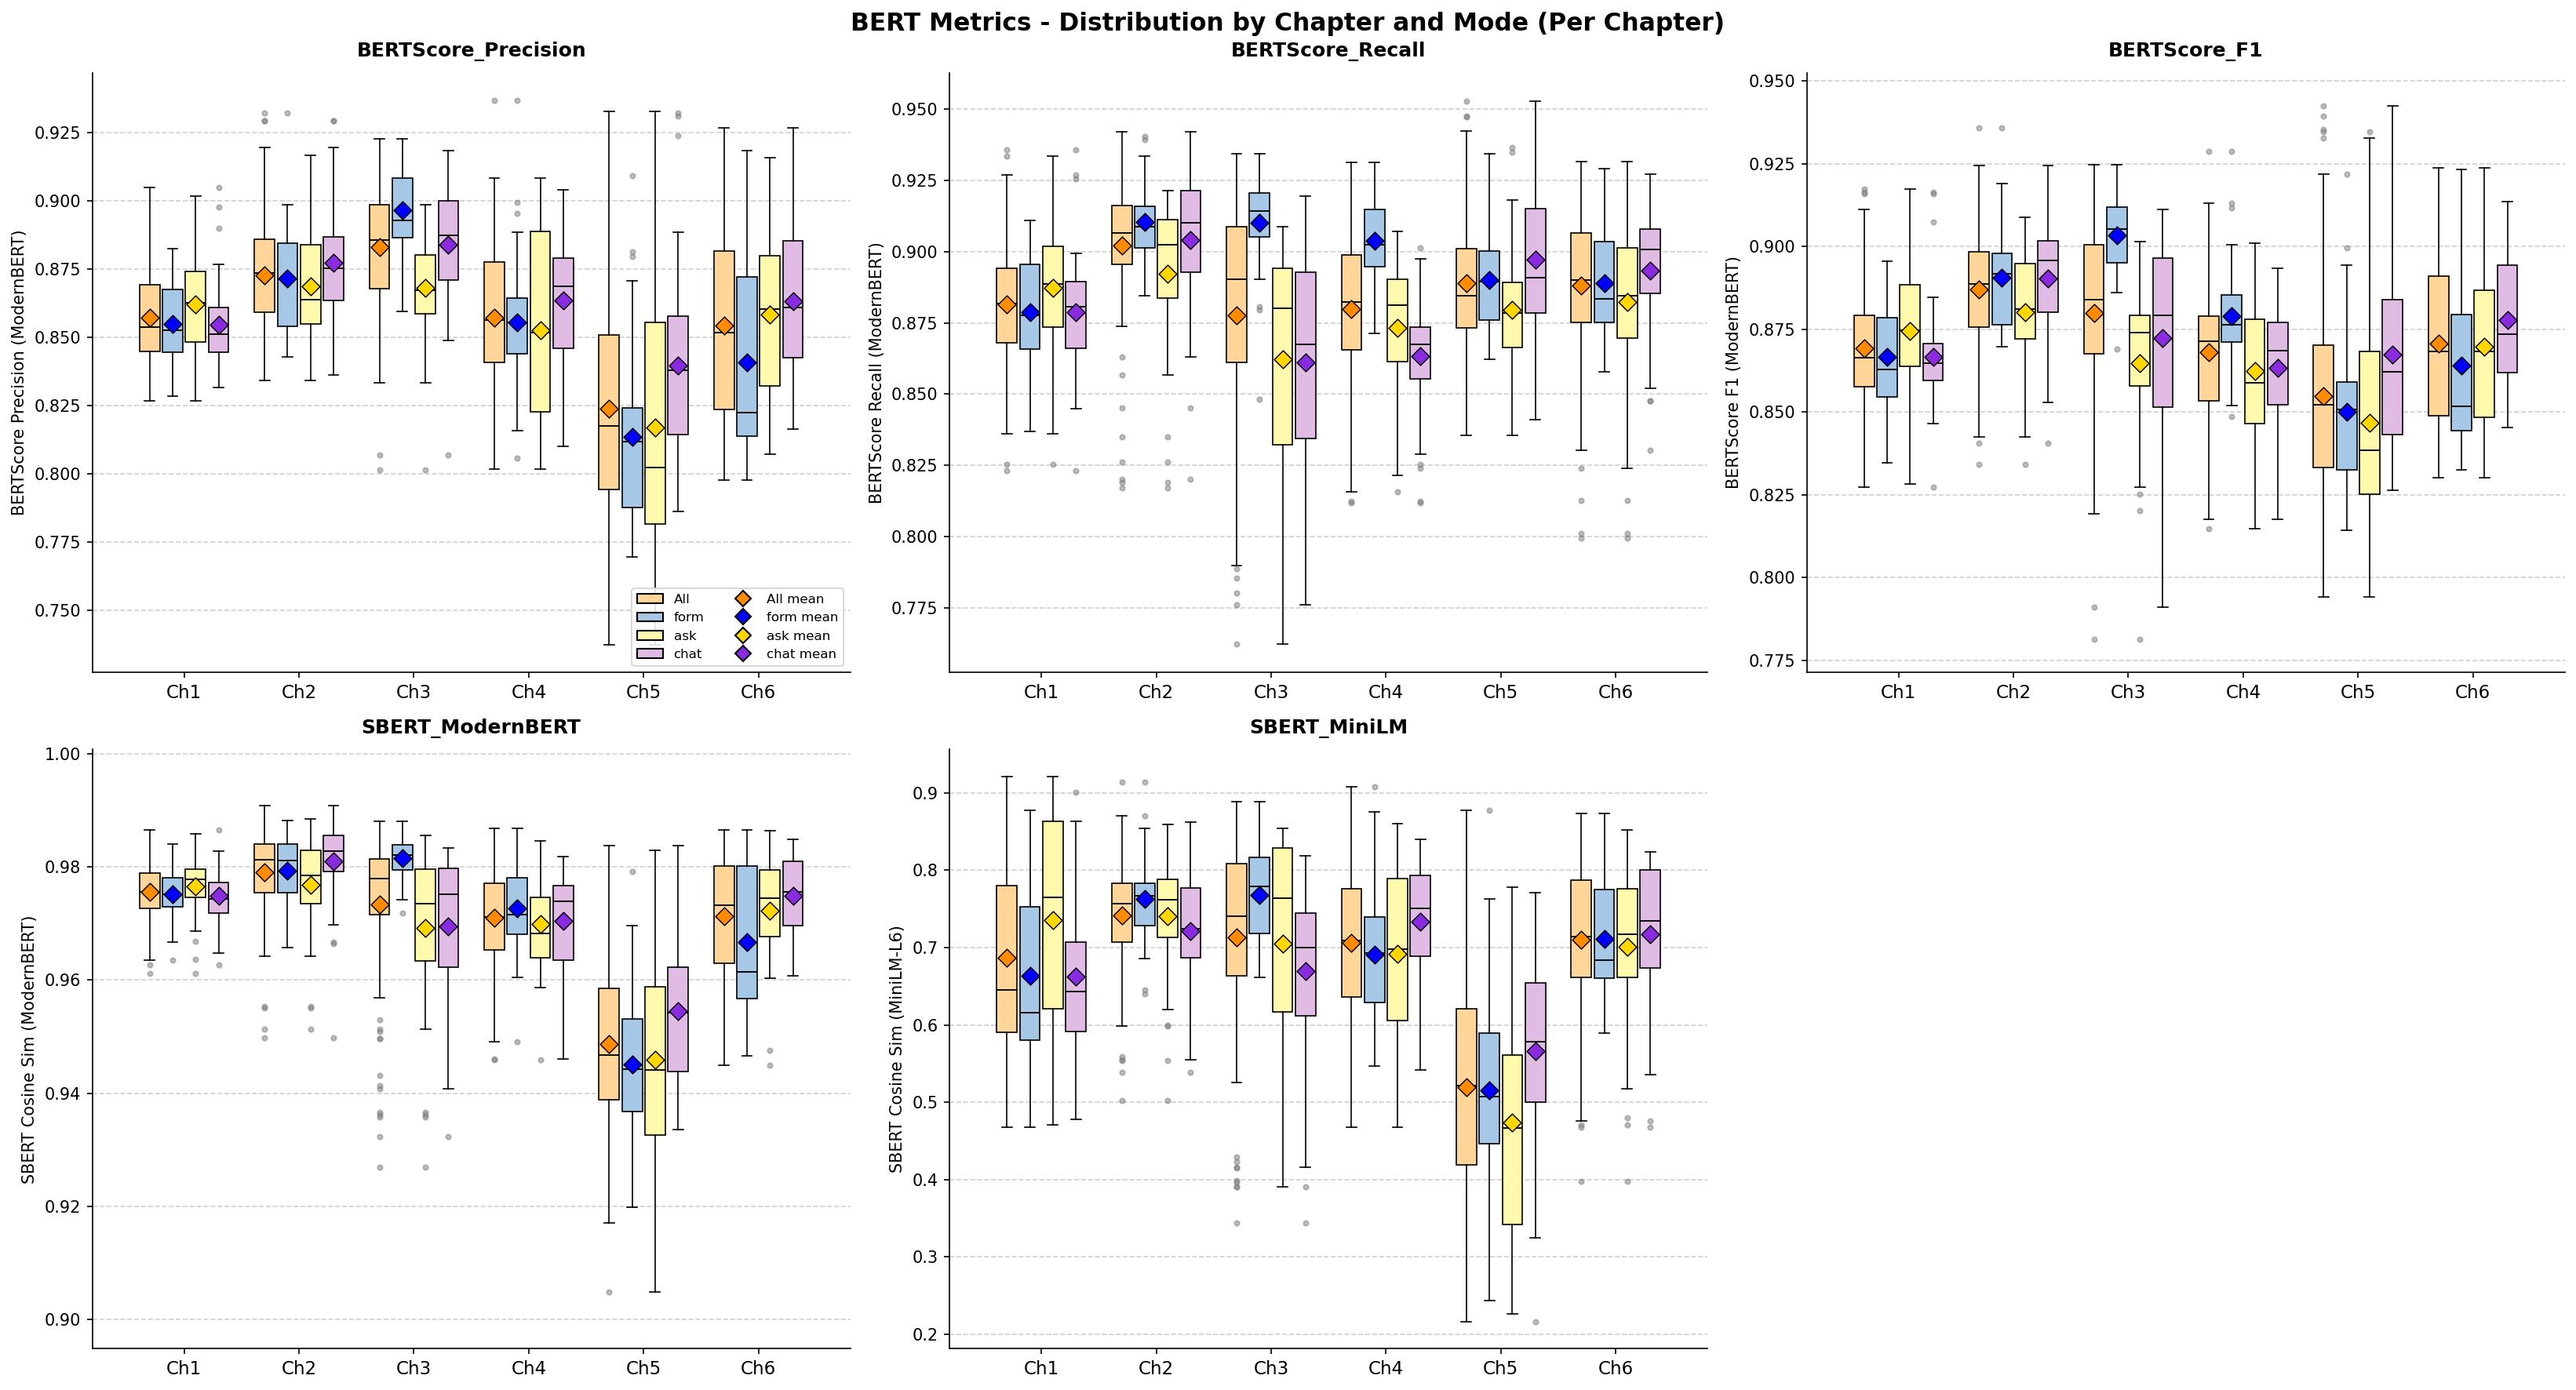
\includegraphics[width=\linewidth,height=0.80\textheight,keepaspectratio]{chapter_bert_metrics_boxplot.png}
\end{frame}

% ============================================================
% Reference: ROPA chapters + AI questionnaire
% ============================================================
\begin{frame}{Reference: ROPA Chapters \& AI Questionnaire}
\footnotesize
\begin{columns}[T]
\begin{column}{0.5\textwidth}
\textbf{The six ROPA chapters} \\[0.05cm]
{\scriptsize (granularity of the chapter-level NLP metrics)}\\[0.12cm]
\begin{enumerate}\setlength{\itemsep}{0.05cm}
  \item Verantwortliche Stelle und Kontaktdaten\\ {\scriptsize\itshape Controller \& contact details}
  \item Zwecke und Rechtsgrundlagen der Verarbeitung\\ {\scriptsize\itshape Purposes \& legal bases}
  \item Kategorien personenbezogener Daten und Datenquellen\\ {\scriptsize\itshape Data categories \& sources}
  \item Betroffene Personen und Empf\"anger\\ {\scriptsize\itshape Data subjects \& recipients}
  \item L\"oschfristen und Aufbewahrungsdauern\\ {\scriptsize\itshape Retention \& erasure periods}
  \item Technische und organisatorische Ma\ss nahmen (TOM)\\ {\scriptsize\itshape Technical \& organizational measures}
\end{enumerate}
\end{column}
\begin{column}{0.5\textwidth}
\textbf{Perceived AI Support questionnaire} \\[0.1cm]
{\scriptsize (6 bespoke items, 5-point Likert: 1 = strongly disagree, 5 = strongly agree)}\\[0.2cm]
\begin{enumerate}\setlength{\itemsep}{0.28cm}
  \item The AI was helpful in creating this document.
  \item The AI helped me to complete the document faster.
  \item I understood why the AI suggested specific GDPR fields.
  \item I trust that the AI made correct suggestions.
  \item I am confident that the AI identified the correct legal basis.
  \item I would use this mode again.
\end{enumerate}
\end{column}
\end{columns}
\end{frame}

% ============================================================
% References
% ============================================================
\begin{frame}[allowframebreaks]{References}
\renewcommand*{\bibfont}{\scriptsize}
\printbibliography[heading=none]
\end{frame}

\end{document}
